%&LaTeX
\documentclass[11pt,a4paper]{article}
\usepackage[frenchb,english]{babel}
\usepackage[applemac]{inputenc}
\usepackage[OT1]{fontenc}
\usepackage[]{graphicx}
\usepackage{amsmath}
\usepackage{amsfonts}
\usepackage{amsthm}
\usepackage{amssymb}
\usepackage{tikz}
\usepackage{mathrsfs}


%\input{8bitdefs}

% marges
\topmargin 10pt
\headsep 10pt
\headheight 10pt
\marginparwidth 30pt
\oddsidemargin 40pt
\evensidemargin 40pt
\footskip 30pt
\textheight 670pt
\textwidth 420pt

\def\imp{\Rightarrow}
\def\gcro{\mbox{[\hspace{-.15em}[}}% intervalles d'entiers 
\def\dcro{\mbox{]\hspace{-.15em}]}}

\newcommand{\be} {\begin{enumerate}}
\newcommand{\ee} {\end{enumerate}}
\newcommand{\deb}{\begin{eqnarray*}}
\newcommand{\fin}{\end{eqnarray*}}
\newcommand{\ssi} {si et seulement si }
\newcommand{\D}{\mathrm{d}}
\newcommand{\Q}{\mathbb{Q}}
\newcommand{\Z}{\mathbb{Z}}
\newcommand{\N}{\mathbb{N}}
\newcommand{\R}{\mathbb{R}}
\newcommand{\C}{\mathbb{C}}
\newcommand{\F}{\mathbb{F}}
\newcommand{\U}{\mathbb{U}}
\newcommand{\re}{\,\mathrm{Re}\,}
\newcommand{\im}{\,\mathrm{Im}\,}
\newcommand{\ord}{\mathrm{ord}}
\newcommand{\Gal}{\mathrm{Gal}}
\newcommand{\legendre}[2]{\genfrac{(}{)}{}{}{#1}{#2}}
%\renewcommand\familydefault{cmss}
\title{Solutions to David A.Cox  "Galois Theory''}
\author{Richard Ganaye}
\refstepcounter{section} \refstepcounter{section} \refstepcounter{section} \refstepcounter{section}
\refstepcounter{section}\refstepcounter{section}\refstepcounter{section}\refstepcounter{section}
\refstepcounter{section}

\begin{document}
\maketitle

\section{Chapter 10 : GEOMETRIC CONSTRUCTIONS}

\subsection{CONSTRUCTIBLE NUMBERS}

\paragraph{Ex. 10.1.1}

{\it In part (a) of Example 10.1.2 we constructed the $x$-axis. In a similar way show that the $y$-axis is constructible. For each step in your construction be sure to say which of $C1,C2,P1,P2$, and $P3$ you are using.
}

\begin{proof}
Let $ \mathscr{C}$ be the set of constructible numbers in $\C$.

Write $C(\gamma,r)$ the circle with center $\gamma \in \C$ and radius $r$.

Starting from $ \{0,1\}$, we obtain by $C1$ the $x$-axis and by $P2$ the point $-1$ at the intersection of $C(0,1)$ with the $x$-axis, so
$$ \{-1,0,1\} \subset {\mathscr{C}}.$$
If $\alpha = -1, \beta = 1$, then $|\beta - \alpha| = 2$, so $C(-1,2)$ and $C(1,2)$ are constructible by $C2$.

Using $P3$, the intersection $C(-1,2) \cap C(1,2)=\{\delta, - \delta\}$ gives the point $\delta = i\sqrt{3}$. The $y$-axis that goes through $0$ and $\delta$ is so constructible by $C1$.

Example 10.1.2(b) shows then that $i \in \C$ is  constructible. 
\end{proof}

\paragraph{Ex. 10.1.2}

{\it Suppose that $\alpha,\beta,\gamma$ are noncolinear and consider the rays $\overrightarrow{\alpha \beta}$ and $\overrightarrow{\alpha \gamma}$ emanating from $\alpha$ that go through $\beta$ and $\gamma$ respectively. We call this the angle formed by $\alpha,\beta,\gamma$. Also assume that $\alpha, \beta,\gamma$ are constructible.
\be
\item[(a)] Prove that there is a constructible number $\delta$ with positive $y$-coordinate such that the angle formed by $\alpha,\beta,\gamma$ is congruent to the angle formed by $0,1,\delta$. As in Exercise 1, each step in the construction should be justified by $C1,C2,P1,P2$, or $P3$.
\item[(b)] Prove that the claim made in Example 10.1.3 that $\zeta_n = e^{2\pi i/n}$ is constructible if and only if a regular $n$-gon can be constructed by straightedge and compass.
\ee
}

\begin{proof}
\be
\item[(a)] $C(\alpha,1)$ is constructible by $C2$. Let $\gamma'$ the intersection point of the line $\alpha \gamma$ with $C(\alpha,1)$, then $\gamma'$ is constructible by $P2$. Let $\eta$ the orthogonal projection of $\gamma'$ on the line $\alpha \beta$. Then $\eta$ is constructible with the usual construction: the circle $C(\gamma',r)$, with $r=  |\gamma' \alpha|$,  has two intersection points $\alpha,\alpha'$ with the line $\alpha \beta$, and the intersection point $\gamma'' \ne \gamma'$ of $C(\alpha,r)$ with $C(\alpha',r)$ is constructible, so is the line $\gamma' \gamma''$, and $\eta$ the intersection of the line $\gamma' \gamma''$ with the orthogonal line $\alpha \beta$. Then the cosine of the angle $(\overrightarrow{\alpha \beta},\overrightarrow{\alpha \gamma})$ is $\pm | \eta \alpha| $.

Write $\xi, \xi'$ the two intersection points of $C(0,| \eta \alpha|)$ with the $x$-axis. The  line passing trough $\xi$ and orthogonal to the $x$-axis intersect $C(0,1)$ in the point $\delta_1 $ with positive $y$-coordinate, and similarly  line passing trough $\xi'$ and orthogonal to the $x$-axis intersect $C(0,1)$ in the point $\delta_2 $ with positive $y$-coordinate, so both are constructible. Then the cosine of the angle formed by $0,1,\delta_1$ is the opposite of the cosine of the angle formed by $0,1,\delta_2$, and equal in absolute value to $ |\eta \alpha|$. So the angle formed by  $0,1,\delta_1$ or $0,1,\delta_2$ is congruent to the angle formed by $\alpha,\beta,\gamma$, so we can take $\delta = \delta_1$ or $\delta = \delta_2$ such that the angle formed by  $0,1,\delta$ is congruent to the angle formed by $\alpha,\beta,\gamma$, and $\delta$ is constructible.

\item[(b)] $\bullet$ If $\zeta_n$ is constructible, so are $1,\zeta_n,\ldots, \zeta_n^{n-1}$ since $\mathscr{C}$ is a subfield of $\C$ (Theorem 10.1.4), and these points are the vertices of a regular $n$-gon.

$\bullet$ Suppose that a regular $n$-gon can be constructed by straightedge and compass. Let $\beta, \gamma$ be two consecutive vertices. Then the center $\alpha$ of the $n$-gon is constructible, and the measure of the angle formed by $\alpha, \beta,\gamma$ has measure $\theta = 2\pi/n$ (see Example 10.1.3).

By part (a), we can construct $\delta$ with positive $y$-coordinate such that the angle formed by $0,1,\delta$ has the same measure $2\pi/n$. The intersection $\zeta$ of the line $0\delta$ with $C(0,1)$ is constructible, and $\arg(\zeta) = 2\pi/n, |\zeta| = 1$, so $\zeta_n = \zeta$ is constructible.
\ee
\end{proof}

\paragraph{Ex. 10.1.3}

{\it This exercise covers the details omitted in the proof of Theorem 10.1.4.
\be
\item[(a)] Let $\alpha,\beta$ be constructible numbers such that $0,\alpha,\beta$ are collinear. Prove that $\alpha+\beta$ is constructible.
\item[(b)] Let $a\in {\mathscr{C}} \cap \{x\in \R\, | \, x>0\}$. Use Figure 2 in the proof of Theorem 10.1.4 to show that $1/a$ is constructible.
\item[(c)] In the proof of Theorem 10.1.4, we showed that ${\mathscr{C}} \cap  \{x\in \R\, | \, x>0\}$ is closed under addition, mutiplication, and multiplicative inverses. Use this to prove that ${\mathscr{C}} \cap \R$ is a subfield of $\R$.
\item[(d)] Prove that the number $\beta$ pictured in (10.1) is constructible (assuming that $r$ is constructible).
\ee
}

\begin{proof}
\be
\item[(a)] Let $D$ be the line passing through $0,\alpha,\beta$, and $C$ the circle of radius $|\beta|$ with center $\alpha$. Then $D$ and $C$ intersect in two points, one of them being $\alpha + \beta$, which is so constructible.
\item[(b)] As $a$ is constructible, so is $ia$. We can construct the parallel to the line $1,ia$ passing through $i$. The intersection point of this parallel with the $x$-axis gives a point $d>0$. As the triangles $(0,d,i)$ and $(0,1,ia)$ are similar, $d/1 = i/ia$, so $1/a = d$ is constructible.
\item[(c)] We have proved in the text that $\mathscr{C}$ is a subgroup of $(\C,+)$, so ${\mathscr{C}} \cap \R$ is a subgroup of $(\R,+)$.

Let $a,b\in {\mathscr{C}} \cap \R$. If $a = 0$ or $b = 0$ then $a+b \in  {\mathscr{C}} \cap \R$. If $a \ne 0, b\ne 0$ then $|a| = \pm a \in {\mathscr{C}} \cap \R_+^*$, so $|ab| = |a| |b| \in  {\mathscr{C}} \cap \R_+^*$, therefore $ab =\pm |ab| \in {\mathscr{C}} \cap \R$.

Let $a \in {\mathscr{C}} \cap \R, a\ne 0$. then $| a | \in {\mathscr{C}} \cap \R_+^*$, so $1/|a| \in {\mathscr{C}} \cap \R_+^*$. Therefore $1/a = \pm 1/|a| \in {\mathscr{C}} \cap \R$.

Conclusion: ${\mathscr{C}} \cap \R$ is a subfield of $\R$.
\item[(d)] We can construct the orthogonal line $D$ to the $x$-axis passing through $1$, the perpendicular bisector of $(0,2)$. As $r$ is constructible, so is $1+r$ (Exercise 10.1.3(a)). The intersection of the perpendicular bisector of $(0,1+r)$ with the $x$-axis gives the number $(1+r)/2$, which is so constructible. The intersection of the circle with radius $(1+r)/2$ centered in $(1+r)/2$ with $D$ give $\beta$ with positive $y$-coordinate, and so $\beta$ is constructible.

The end of the proof of Theorem 10.1.4 shows that $\sqrt{r}$ is constructible.
\ee
\end{proof}

\paragraph{Ex. 10.1.4}

{\it This exercise covers the details omitted in the proof of Theorem 10.1.6.
\be
\item[(a)] Suppose that a line $l_1$ goes through distinct points $\alpha_1 = u_1+iv_1$ and $\beta_1 = u_2+iv_2$, where $u_1,v_1,u_2,v_2$ lie in a subfield $F \subset \R$. Prove that $l_1$ is defined by an equation of the form $a_1x +b_1y = c_1$ where $a_1,b_1,c_1 \in F$.
\item[(b)] Suppose that $\alpha_2 \ne \beta_2$ and $\gamma_2$ are complex numbers whose real and imaginary parts lie in a subfield $F\subset \R$. Prove that the circle $C$ with center $\gamma_2$ and radius $|\alpha_2-\beta_2|$ has an equation of the form (10.3) with $a_2,b_2,c_2 \in F$.
\item[(c)] In the proof of Theorem 10.1.6, we considered the equations (10.2) and (10.3) when $a_1\ne 0$. Explain what happens when $a_1 = 0$ in (10.2).
\ee
}

\begin{proof}
\be
\item[(a)]
 Let $M = (x,y),A = (u_1,v_1),B = (u_2,,v_2)$ the points of $\R^2$ with affixes $z,\alpha_1,\beta_1$, where $\alpha_1\ne \beta_1$.
Then 
\begin{align*}
M \in (AB) &\iff \det(\overrightarrow{AM}, \overrightarrow{AB}) = 0\\
&\iff
\left|
\begin{array}{ccc}
  x-u_1& u_2-u_1    \\
  y-v_1& v_2-v_1      
\end{array}
\right|
=0\\
&\iff (v_2-v_1)x - (u_2-u_1)y -u_1(v_2-v_1) +v_1 (u_2-u_1) = 0\\
&\iff a_1x+b_1y = c_1
\end{align*}
where $a_1 = v_2-v_1, b_1 = -(u_2-u_1), c_1 = u_1(v_2-v_1) - v_1(u_2-u_1) \in F$.
\item[(b)] Let $z = x+iy, \gamma_2 = u+iv, \alpha_2 - \beta_2 = a +ib$, where $u,v,a,b \in F$. Then
\begin{align*}
z \in C &\iff |z-\gamma_2|^2 = |\alpha_2-\beta_2|^2\\
&\iff(x-u)^2 + (y-v)^2 = a^2+b^2\\
&\iff x^2+y^2+a_2x+b_2y+c_2 = 0,
\end{align*}
where $a_2 = -2u,b_2 = -2v ,c_2 = -(a^2+b^2) \in F$.
\item[(c)] If $a_1 = 0$, then for all $z =x+iy \in l$, $y=c_1/b_1 x = ux$, where $u = c_1/b_1 \in F=F_n$. Substituting $y = ux$ into (10.3) gives the quadratic equation
$$x^2+a_2x+u^2x^2+b_2ux+c_2.$$
Therefore $x$ lies in a quadratic extension $F_{n+1}$ of $F_n$ (and $y \in F_n \subset F_{n+1}$).
\ee
\end{proof}

\paragraph{Ex. 10.1.5}

{\it In this exercise you will give two proof that $\zeta_3 = e^{2\pi i/3}$ is constructible.
\be
\item[(a)] Give a direct geometric construction of $\zeta_3$ with each step justified by citing $C1,C2,P1,P2$ or $P3$.
\item[(b)] Use Theorem 10.1.6 to show that $\zeta_3$ is constructible.
\ee
}

\begin{proof} 
\be
\item[(a)]
As $\mathrm{Re}(\zeta_3) = -1/2$, $\zeta_3$ is on the perpendicular bisector of $(-1,0)$.

We gives the details of the construction:
$C(0,1)$ and $C(-1,0)$ are constructible by $C2$, so the two intersection points are constructibles by $P3$, and these two points are $\zeta_3,\overline{\zeta}_3$, so $\zeta_3$ is constructible.
\item[(b)] As the minimal polynomial of $\zeta_3$ over $\Q$ is $x^2+x+1$, the extension $\Q\subset \Q(\zeta_3)$ is quadratic, so $\zeta_3$ is constructible by Theorem 10.1.6.
\ee
\end{proof}



\paragraph{Ex. 10.1.6}

{\it Show that it is impossible to trisect a 60� angle by straightedge and compass.
}

\begin{proof} If  a 20� angle was constructible by straightedge and compass, then $\zeta_{18}$ would be constructible. The minimal polynomial of $\zeta_{18}$ is $\Phi_{18}(x)$.

By Exercise 9.1.12, $\Phi_{18}(x) = \Phi_9(-x)$, and $\Phi_9(x) = \Phi_3(x^3) = x^6 +x^3+1$, so
$$\Phi_{18}(x) = x^6-x^3+1.$$
Therefore $[\Q(\zeta_{18}) : \Q] = 6$. If $\zeta_{18}$ was constructible, by Theorem 10.1.6, there exist subfields 
$$\Q = F_0 \subset F_1\subset \cdots \subset F_{n-1}\subset F_n \subset \C,$$
with $[F_i:F_{i-1}] = 2$ for $1\leq i \leq n$, and $\zeta_{18} \in F_n$. But then by the tower theorem, $6 = [\Q(\zeta_{18}) : \Q] $ divides $[F_n : \Q] = 2^n$, and $3 \mid 2^{n-1}$: this is a contradiction. So $\zeta_{18}$ is not constructible, hence it is impossible to trisect a 60� angle by straightedge and compass.
\end{proof}

\paragraph{Ex. 10.1.7}

{\it Suppose we have extensions $\Q\subset F \subset \C$ where $[F:\Q]$ is finite. Prove that there is a field $M$ such that $F \subset M \subset \C$ and $M$ is a Galois closure of $F$ over $\Q$.
}

\begin{proof}
As $[F:\Q]$ is a finite extension, and as $\Q$ has characteristic 0, by the Theorem of the Primitive Element (Corollary 5.4.2 (b)), $F = \Q(\alpha)$ for some $\alpha \in F$. Let $f$ be the minimal polynomial of $\alpha$ over $\Q$.

As $\C$ is an algebraically closed field, $f$ splits completely over $\C$. Let $\alpha_1=\alpha,\alpha_2,\ldots,\alpha_n$ the roots of $f$ in $\C$, and $M = \Q(\alpha_1,\ldots,\alpha_n)$ the splitting field of $f$ in $\C$. Then
\be
\item[(a)] $\Q \subset M$ is a Galois extension, since the splitting field of $f$ over $\Q$ is a normal extension of $\Q$, and separable since the characteristic of $\Q$ is 0.
\item[(b)] Let $M \subset M'$ by any other extension such that $M'$ is a Galois extension over $\Q$. As $\alpha \in M \subset M'$ is a root of $f$ and as $M'$ is normal, $f$ splits completely over $M'$, with roots $\beta_1 = \alpha_1,\beta_2,\ldots,\beta_n, \in M'$. Let $M'' = \Q(\beta_1,\ldots,\beta_n)$, so $M''$ is a splitting field of $f$ over $\Q$. By the uniqueness of splitting fields (Corollary 5.1.7), there is an isomorphism $\varphi:M\to M''$ that is the identity on $L$. Since $M'' \subset M'$, $\varphi$ defines a field homomorphism $\varphi:M \to M'$.
\ee
So the parts (a),(b) of the definition of an Galois closure are satisfied.

Conclusion: there is a field $M$ such that $F \subset M \subset \C$ and $M$ is a Galois closure of $F$ over $\Q$.
\end{proof}

\paragraph{Ex. 10.1.8}

{\it In the Mathematical notes we defined the field ${\mathscr P} \subset \R$ and what it means for a subfield $F \subset \R$ to be Pythagorean.
\be

\item[(a)] Let $\alpha$ be a real number. Prove that $\alpha \in {\mathscr P} $ if and only if there is a sequence of fields $\Q = F_0\subset \ldots \subset F_n \subset \R$ such that $\alpha \in F_n$, and for $i=1,\ldots,n$ there are $a_i,b_i \in F_{i-1}$ such that $F_i = F_{i-1}\left(\sqrt{a_i^2+b_i^2}\right)$.
\item[(b)] Prove that ${\mathscr P} $ is the smallest Pythagorean subfield of $\R$.
\ee
}

Write $\mathbb{P}$ the set of points of $\C$ (identified with the Euclidean plane) constructible by a sequence of straightedge-and-dividers constructions, and $\mathbb{D}$ the set of lines passing through two distinct such points (so constructible by straightedge-and-dividers) .

\bigskip

{\bf Lemma 1. } {\it If $A,B,C\in {\mathbb P}$, with $A\ne B$, then the parallel $l$ to $(AB)$ passing through $C$ is in $\mathbb{D}$.}
\begin{proof} Let $C'$ the symmetric point of $C$ relative to $A$, and $C''$ the symmetric point of $C'$ relative to $B$, so $\overrightarrow{AC'} = -\overrightarrow{AC}, \overrightarrow{BC''} = - \overrightarrow{BC'}$. Since $AC = AC'$ and $BC' = BC''$, $C',C''$ lie in  $\mathbb{P}$, and $\overrightarrow{CC''} = 2 \overrightarrow{AB}$, so $C \ne C''$ and $(CC'')$ is parallel to $(AB)$, with $(CC'') \in \mathbb{D}$. So $l = (CC'') \in \mathbb{D}$.
\end{proof} 

{\bf Lemma 2.}  ${\mathscr P} $ {\it is a subfield of $\R$.}
\begin{proof}
Using Lemma 1, we can mimic the proof of first part of Theorem 10.1.4.
\end{proof}

{\bf Lemma 3.} {\it Let $\alpha = a+ib \in \C$, where $a,b \in \R$. Then $\alpha \in \mathbb{ P}$ if and only if $a,b \in {\mathscr P} $.}

%{\it  Let $l = (AB),\  A,B \in \mathbb{P}$, a straightedge-and-dividers constructible line, and $C \in \mathbb{P}$ a straightedge-and-dividers constructible point. Then line $l'$ passing trough $C$ and orthogonal to $l$ is a straightedge-and-dividers constructible line: $l' \in \mathbb{D}$.}

\begin{proof}

\be

\item[$\bullet$] Suppose that $\alpha =a +i b \in \mathbb{P}$. By Lemma 1, we can construct by straightedge-and-dividers constructions the lines passing through $\alpha$ and parallel to the axis, so $a, ib$ are constructible, and using the divider, so are  the real numbers $a,b$, therefore $a,b \in {\mathscr P} $.
\item[$\bullet$] Suppose that $a,b \in {\mathscr P} $. Then $a, ib \in \mathbb{P}$, and the intersection $\alpha = a+ib$ of the lines passing through these two points and parallel to the $y$-axis and $x$-axis respectively lies in $\mathbb{P}$.
\ee

\end{proof}


\begin{proof} (Ex. 10.1.8)
\be
\item[(a)] Let $\alpha$ be a real number.
\be
\item[$\bullet$]  Suppose that there is a sequence of fields $\Q = F_0\subset \ldots \subset F_n \subset \R$ such that $\alpha \in F_n$, and for $k=1,\ldots,n$, there are $a_k,b_k \in F_{k-1}$ such that $F_k= F_{k-1}\left(\sqrt{a_k^2+b_k^2}\right)$.

We prove by induction that $F_k \subset {\mathscr P} $. Since ${\mathscr P} $ is a subfield of $\R$, $F_0 = \Q \subset \mathscr{P}$. Suppose that $F_{k-1} \subset {\mathscr P} $. As $a_k,b_k\in F_{k-1} \subset {\mathscr P} $, $\sqrt{a_k^2+b_k^2} \in {\mathscr P} $ (see the Mathematical Notes), so $F_k=F_{k-1}\left(\sqrt{a_k^2+b_k^2}\right) \subset {\mathscr P} $, and the induction is done. 

Therefore  $F_n \subset {\mathscr P} $, and $\alpha \in F_n$, so $\alpha \in {\mathscr P} $. 

\item[$\bullet$]  Conversely, suppose that $\alpha = a+ib \in {\mathbb P}$. We use induction on the number $N$ of steps in the construction of $\alpha$ to prove that there is a sequence of subfields of $\R$, $\Q = F_0\subset \ldots \subset F_n \subset \R$, such that $a,b \in F_n$, where $F_k= F_{k-1}\left(\sqrt{a_k^2+b_k^2}\right),\ k=1,\ldots,n$.

 When $N = 0$, we must have $\alpha = 0,1$ or $i$, in which case $F_n = F_0 = \Q$ contains the real and imaginary part of $\alpha$.

Now suppose that $\alpha$ is constructed in $N\geq1$ steps, where the last step use the intersection of two lines $l_1,l_2$. As in the proof of the Theorem 10.1.6, the coordinates of $\alpha$ lie in the same field $F_n$.

If the last step uses the divider, then their exists four points $\beta,\gamma, \delta, \varepsilon \in \mathbb{P}$ such that $\delta,\varepsilon, \alpha$ are collinear and $|\alpha - \delta| = |\beta - \gamma|$. Moreover, by the induction hypothesis,  the coordinates $\beta_x, \beta_y,\gamma_x,\ldots$ of $\beta,\gamma,\delta,\varepsilon$ are in $F_n$.

Then $\alpha - \delta = \lambda(\varepsilon - \delta), \lambda \in \R$, with
$$\lambda = \pm \frac{|\alpha - \delta|}{|\varepsilon - \delta|}=\pm \frac{|\beta - \gamma|}{|\varepsilon - \delta|}.$$
Let 
\begin{align*}
F_{n+1} &= F_n(|\beta - \gamma|) = F_n(\sqrt{s^2+t^2}), \mathrm{where}\  s = \beta_x - \gamma_x , t = \beta_y - \gamma_y \in F_n,\\
F_{n+2} &=F_{n+1}(|\varepsilon - \delta|) = F_{n+1}(\sqrt{u^2+v^2}),  \mathrm{where}\  u = \varepsilon_x - \delta_x, v = \varepsilon_y - \delta_y \in F_n.
\end{align*}
Then $\lambda \in F_{n+2}$. As $\alpha = a+ i b =  \delta + \lambda (\varepsilon - \delta)$, $a, b \in F_{n+2}$, and the induction is done.

In particular, if $\alpha = a+ib \in {\mathscr P}  = \mathbb{P} \cap \R$, then $b=0, \alpha = a \in F_n$, where 
$\Q = F_0\subset \ldots \subset F_n \subset \R$ and there are $a_k,b_k\in F_{k-1}$ such that $F_k = F_{k-1}\left(\sqrt{a_k^2+b_k^2}\right),\ k= 1,\ldots,n$.
\ee

\item[(b)] By the Mathematical notes, if $a,b \in {\mathscr P} $, then $\sqrt{a^2+b^2} \in {\mathscr P} $, so $\mathscr P$ is a Pythagorean subfield of $\R$.

Let $K$ any Pythagorean subfield of $\R$, and take any $ \alpha \in {\mathscr P} $.  By part (a), there exists a sequence of subfields of $\R$,
$$\Q = F_0\subset \ldots \subset F_n \subset \R,$$
such that $\alpha \in F_n$, and for $k=1,\ldots,n$ there are $a_k,b_k \in F_{k-1}$ such that $F_k= F_{k-1}\left(\sqrt{a_k^2+b_k^2}\right)$.
As any subfield of $\R$, $K$ contains $\Q$, so $F_0 = \Q \subset K$.

By induction, suppose that $F_{k-1} \subset K$ for some integer $k, 1 \leq k\leq n$. Then $F_k = F_{k-1}(\sqrt{a_k^2+b_k^2})$, where $a_k,b_k\in F_{k-1} \subset K$. As $K$ is Pythagorean, $\sqrt{a_k^2+b_k^2} \in K$, so $F_k \subset K$, and the induction is done.

So $F_n \subset K$, and $\alpha \in F_n$, so $\alpha \in K$. Hence ${\mathscr P}  \subset K$, so $\mathscr P$ is the smallest Pythagorean subfield of $\R$.
\ee
\end{proof}

\paragraph{Ex. 10.1.9}

{\it Show that the lune illustrated in the Historical Notes has the same area as the triangle $AOB$ in the illustration.
}

\begin{proof}
Let $l = OA=OB$ be the side of the triangle $OAB$, and $A = l^2/2$ the area of this triangle. 

The area of the semicircle with diameter $AB$ is $$A_1 = \frac{1}{2} \pi \left(\frac{\sqrt{2}}{2} l \right)^2 = \frac{\pi}{4} l^2.$$
The area of the quarter circle with radius $0A$ is $\frac{\pi}{4} l^2,$
so the area between the arc $AB$ and the chord $AB$ is $$A_2 = \frac{\pi}{4} l^2 - A.$$
Therefore the area of the lune, the shaded region of the figure in historical notes, is
$$A_1 - A_2 = \frac{\pi}{4} l^2 -  \left(\frac{\pi}{4} l^2 - A\right) = A,$$
so is this area is the area $A = l^2/2$ of the triangle.
\end{proof}

\paragraph{Ex. 10.1.10}

{\it The quadratrix is the curve $y = x \cot(\pi x/2)$ for $0<x\leq 1$. In this problem, you will use this curve to square the circle and trisect the angle.
\be
\item[(a)] Show that $2/\pi = \lim_{x\to 0^+} x \cot(\pi x/2)$, i.e., the quadratrix meets the $y$ axis at $y = 2/\pi$. We will follow Hippias and include this point in the curve.
\item[(b)] Show that we can square the circle starting from 0 and 1 and constructing new points using $C1,C2,P1,P2$, or $P3$, together with the intersections of constructible lines with the quadratrix.
\item[(c)] A point $(a,b)$ on the quadratrix determines an angle $\theta$ as pictured below (see fig. in Cox p. 269). Prove that $\theta = \pi a/2$.
\item[(d)] Suppose that we are given an angle $0 < \theta < \pi/2$. Prove that we can trisect $\theta$ starting from 0,1, and $\theta$ and constructing new points using $C1,C2,P1,P2$, or $P3$, together with the intersections of constructible lines with the quadratrix.
\item[(e)] Explain how the method of part (d) can be adapted to trisect arbitrary angles.
\item[(f)] Using the quadratrix, what else can you do to angles besides trisecting them?
\ee
}

\begin{proof}
\be
\item[(a)] For all $x \in ]0,\pi]$,
$$x \cot\left(\frac{\pi x}{2}\right) = \frac{2}{\pi}\,  \frac{{\frac{\pi x}{2}}}{{\sin\left(\frac{\pi x}{2}\right)}}\,  \cos \left(\frac{\pi x}{2}\right).$$
As $\lim_{u\to 0} \frac{\sin u}{u} = 1$ and $\lim_{u\to 0} \cos(u)=1$, then
$$\lim_{x \to 0} x \cot\left(\frac{\pi x}{2}\right) = \frac{2}{\pi}.$$

\item[(b)]
 Let $\mathbb{H} $ be the set of Hippias-constructible points. Then by Section 10.1, $\mathbb{H}$ is a subfield of $\C$, and ${\mathscr{C}}$ is a subfield of $\mathbb{H}$.

As $(0,2/\pi)$ is on the quadratrix and the $y$-axis is constructible,  $(2/\pi) i \in \mathbb{H}$. Since $i$ is constructible and since $\mathbb{H}$ is a field, $2/\pi \in \mathbb{H}$, so $\pi/2$ and $\pi$ are in $\mathbb{H}$. 
Then the proof of Theorem 10.1.4 shows that $\sqrt{\pi}\in \mathbb{H}$. If $r \in \R_+^*$ is a constructible number and the radius of a circle $C$, then $\sqrt{\pi} r \in \mathbb{H}$, so we can square every constructible circle with the quadratrix.

\item[(c)] As $M = (a,b)$ is on the quadratrix, $b = a \cot (\pi a/2)$. By definition, $\theta$ is a measure of the angle $\widehat{(\overrightarrow{OM}, \vec{e}_2)}$ (where $\vec{e}_2 = (0,1)$), then 
$$\frac{b}{a} = \cot \theta = \cot\left(\frac{\pi}{2} a\right).$$
If $\theta = 0$, then $a = 0$. Since the restriction $\cot :\,  ]0, \pi/2] \to [0,+\infty[$ is strictly decreasing, hence is injective, and $\theta \in ]0, \pi/2], \frac{\pi}{2} a \in ]0, \pi/2]$, then 
$$\theta = \frac{\pi}{2} a,\qquad 0 \leq a \leq 1.$$

\item[(d)]
Let $l$ a line containing the origin $O$, and $(a,b)$ the intersection of $l$ with the quadratrix. As in part (c),
$$\frac{b}{a} = \cot \theta = \cot\left(\frac{\pi}{2} a\right).$$
Let $(c,d)$ be the point on the quadratrix corresponding with the angle $\theta/3$. Then
$$\frac{d}{c} = \cot \left( \frac{\theta}{3} \right) = \cot\left(\frac{\pi}{2} c\right),$$
therefore, as in part (c), $\frac{\theta}{3} = \frac{\pi}{2} c$, so
$$c = \frac{a}{3}.$$
Starting from the line $l$, the quadratrix and the points $0,1$, We can construct with straightedge-and-compass $M=(a,b)$, and $c =a/3$ by the construction of Section 10.1, Figure 1, thus we can construct $M' = (c,d)$ at the intersection of the quadratrix and the vertical line passing through $(c,0)$, and this gives the constructive line $l' = OM'$ corresponding to the angle $\theta/3$. So we can trisect every angle $\widehat{(\overrightarrow{OM}, \vec{e}_2)}$, with measure $\theta,\ 0 < \theta <  \pi /2 $. 

\item[(e)]
Using construction given in Exercise 2 (a), we can transport with straightedge-and-compass constructions any given angle determined by  $\alpha,\beta,\gamma$ (with measure $\theta,\ 0 < \theta <  \pi /2 $) on a congruent angle $\widehat{(\overrightarrow{OM}, \vec{e}_2)}$. The inverse transport gives the trisection of the given angle.
If $\pi/2 \leq \theta \leq \pi$ (obtuse angle), then we can trisect the constructive angle with measure $\theta - \pi/2$, the add the constructive angle with measure $\pi/6$. So we can trisect arbitrary angle with the quadratrix.

\item[(f)] In the reasoning of parts(d) and (e), we can replace $\theta/3$ by $\theta/n$, where $n$ is any positive integer. So we can divide any angle in $n$ parts with the quadratrix. Thanks to the quadratrix!
\ee
\end{proof} 

\paragraph{Ex. 10.1.11}

{\it Explain how the points of intersection of the parabolas $y=x^2$ and $x=y^2$ enable one to duplicate the cube. Your explanation should include a picture.
}

\begin{proof}
Let $(a,b)$ the intersection point (other than (0,0)) at the intersection of the two parabolas $y =x^2$ and $x = 2y^2$. Then $ a^2 = b, a = 2 b^2$. Multiplying these two equalities, we obtain
$$a^3 = 2 b^3.$$
The volume of the cube with side $a$ is twice the volume of the cube of side $b$.
\end{proof}

\paragraph{Ex. 10.1.12}

{\it The spiral of Archimedes is the curve whose polar equation is $r = \theta$.
\be
\item[(a)] Explain how the spiral and $\theta = \pi/2$ enable one to square the circle.
\item[(b)] Given an angle $\theta_0$, explain how the spiral enables one to trisect $\theta_0$.
\ee
}

\begin{proof}
\be
\item[(a)] If $M =(x,y)$ is a point of the spiral of Archimedes, then
$$r =\sqrt{x^2+y^2} = \theta.$$
If $\theta = \pi /2$, then $x = 0, y>0$, so $y = \pi/2$.
So $\pi/2$ and $\pi$ is constructible, if we use the spiral of Archimede, and also $\sqrt{\pi}$ by Section 10.1. So the spiral of Archimedes enables one to square the circle.

\item[(b)] If $0 < \theta_0 < \pi$, let $M=(a,b)$ the corresponding point on the spiral, so $$r = \sqrt{a^2+b^2} = \theta_0.$$ We can obtain by the geometric construction of Section 10.1 the real number $r' = r/3$. Let $C$ the circle with center 0 and radius $r' = r/3$. The intersection of $C$ with the spiral gives is the point $M' = ((r/3)\cos(\theta_0/3),(r/3)\sin(\theta_0/3))$, so the measure of the angle $\widehat{(\vec{e}_1,\overrightarrow{OM'})}$ is $\theta_0 /3$. So the spiral enables one to trisect $\theta_0$. 
\ee
\end{proof}

\subsection{REGULAR POLYGONS AND ROOTS OF UNITY}

\paragraph{Ex. 10.2.1}

{\it Suppose that $2^k+1$ is an odd prime. Prove that $k$ is a power of 2.
}

\begin{proof}Let $N = 2^k + 1, \ k\geq 1$ an odd prime. Suppose that there exists an odd divisor $q$ of $k$, so $k = ql$. Since $l$ is odd,
$$2^k+1 =2^{ql}+1 = (2^q + 1)(2^{q(l-1)} - 2^{q(l-2)}+ \cdots -2^q + 1) = (2^q+1)\sum_{j=0}^{l-1} (-1)^j 2^{qj},$$
so $2^q + 1$ divides $2^k+1$, and $1\leq q \leq k$, hence $ 1< 3 \leq 2^q + 1 \leq 2^k < 2^k+1$, so $2^q + 1$ is a nontrivial divisor of $N = 2^k+1$. Therefore $N$ is composite: this is a contradiction.

 Thus $k$ has no odd divisor, so $k = 2^n$ for some integer $n$, and $N = 2^{2^n}+ 1$ is a Fermat prime.
\end{proof}

\paragraph{Ex. 10.2.2}

{\it Let $p$ be prime. In Example 9.1.6, we showed that
$$\Phi_{p^2}(x) = x^{p(p-1)}+ x^{p(p-2)} + \cdots + x^{2p} +x^p + 1.$$
The goal of this exercise is to prove that $\Phi_{p^2}(x)$ is irreducible over $\Q$ using only the Sch�nemann-Eisenstein criterion.
\be
\item[(a)] Explain how the formulas of Example 9.1.6 imply that
$$(x+1)^{p^2} - 1 = ((x+1)^p - 1)\Phi_{p^2}(x+1).$$
\item[(b)] Let $\overline{\Phi}_{p^2}(x+1)$ be the reduction of $\Phi_{p^2}(x+1)$ modulo $p$. Show that
$$x^{p^2} = x^p\, \overline{\Phi}_{p^2}(x+1).$$
\item[(c)] Show that $\Phi_{p^2}(x+1)$ is irreducible over $\Q$ by the Sch�nemann-Eisenstein criterion. As in the proof of Proposition 4.2.5, this will imply that the same is true for $\Phi_{p^2}(x)$.
\ee
}

\begin{proof} (Ex 10.2.2)
\be
\item[(a)] As in Example 9.1.6, using Proposition 9.1.5, we obtain
$$x^p -1 = \Phi_1(x) \Phi_p(x) \quad \mathrm{and} \quad x^{p^2} - 1 = \Phi_1(x) \Phi_p(x) \Phi_{p^2}(x).$$
Thus
$$x^{p^2} - 1 = (x^p-1) \Phi_{p^2}(x).$$
The substitution $x \to x+1$ gives
$$(x+1)^{p^2} - 1 = ((x+1)^p - 1)\Phi_{p^2}(x+1).$$

\item[(b)]
We know that $p \mid \binom{p}{k}, \ 1 \leq k \leq p-1$, so
$$(x+1)^p  \equiv x^p + 1 \pmod p $$
Therefore
$$ (x+1)^{p^2} =[(x+1)^p]^p  \equiv  (x^p + 1)^p \equiv x^{p^2} \pmod p.$$
The reduction modulo $p$ of the equality proved in part (a) gives
$$x^{p^2} = x^p\, \overline{\Phi}_{p^2}(x+1).$$

\item[(c)] As $ \overline{\Phi}_{p^2}(x+1) = x^{p^2-p}$, all the the coefficients of $\Phi_{p^2}(x+1)$ are divisible by $p$, except the leading coefficient. Moreover $\Phi_{p^2}(1) = p$, so the constant coefficient of $\Phi_{p^2}(x+1)$ is not divisible by $p^2$, so the Sch�nemann-Eisenstein criterion shows that $\Phi_{p^2}(x+1)$ is irreducible over $\Q$, and this is equivalent to the irreducibility of $\Phi_p(x)$ over $\Q$.
\ee
\end{proof}

\paragraph{Ex. 10.2.3}

{\it Using only Proposition 4.2.5, Theorem 10.1.12, and Exercise 1, show that $\zeta_p$ is constructible if and only if $p$ is a Fermat prime.
}

\begin{proof} 
Here we suppose that $p$ is an odd prime.

The splitting field of $\Phi_p$ over $\Q$ is $L = \ \Q(\zeta_p,\zeta_p^2,\ldots,\zeta_p^{p-1}) =\Q(\zeta_p)$. As $\Phi_p(\zeta_p) = 0$, and as $\Phi_p(x)$ is irreducible over $\Q$ (Proposition 4.2.5), $\Phi_p$ is the minimal polynomial of $\zeta_p$ over $\Q$, hence
$$[L : \Q] = [\Q(\zeta_p) : \Q] = \deg(\Phi_p) = p-1.$$

\be
\item[$\bullet$] Suppose that $p$ is a Fermat prime, so $p=2^n +1$, where $n=2^k, k\in \N$. Then $[L:\Q] = 2^n$, where $L$ is the splitting field of $\Phi_p$ over $\Q$. By the authorized Theorem 10.1.12, $\zeta_p$ is constructible.

\item[$\bullet$]  Conversely, if we suppose that $\zeta_p$ is constructible, by the same Theorem 10.1.12, $[L:\Q] = 2^n$ for some integer $n\geq 0$, so $p=2^n+1$. As $p$ is prime, by Exercise 1, $p=2^k,\ k\in \N$, so $ = 2^{2^k}+1$ is a Fermat prime.
\ee
Conclusion: if $p$ is an odd prime, $\zeta_p$ is constructible if and only if $p$ is a Fermat prime.
\end{proof}

\paragraph{Ex. 10.2.4}

{\it Prove that $$(\zeta_n)^{\frac{n}{m}} = \zeta_m$$ when $m\mid n, \ m>0$, and use this to conclude that if $\zeta_n$ is constructible and $m\mid n,\ m>0$, then $\zeta_m$ is constructible.
}

\begin{proof} 
\be
\item[$\bullet$]  Suppose that $m \mid n,\ m>0$. Since $n/m$ is an integer,
$$(\zeta_n)^{\frac{n}{m}} = \left ( e^{\frac{2\pi i}{n}} \right )^{\frac{n}{m}} = e^{\frac{n}{m} \frac{2\pi i}{n}} = e^{\frac{2\pi i}{m}} = \zeta_m.$$
\item[$\bullet$] If $\zeta_n$ is constructible, and $m\mid n, m>0$, by part (a)
$$\zeta_m = (\zeta_n)^{\frac{n}{m}} $$
is a power of $\zeta_n$. 

As the set of constructible points is a subfield of $\C$, $\zeta_m$ is constructible.
\ee
\end{proof}

\paragraph{Ex. 10.2.5}

{\it Suppose that $n = 2^s p_1\cdots p_r$, where $p_1,\ldots,p_r$ are distinct Fermat primes. Then $\zeta_{p_i}$ is constructible by Exercise 3.
\be
\item[(a)] Show that $\zeta_{2^s}$ is constructible.
\item[(b)] Assume that $\zeta_a,\zeta_b$ are constructible and $\gcd(a,b) = 1$. Prove that $\zeta_{ab}$ is constructible.
\item[(c)] Conclude that $\zeta_n$ is constructible, since $\zeta_{2^s},\zeta_{p_1},\ldots, \zeta_{p_r}$ are.
\ee
}

\begin{proof}
\be
\item[(a)] The minimal polynomial of $\zeta_{2^s}$ over $\Q$ is $\Phi_{2^s}(x)$, and $$\deg(\Phi_{2^s}(x)) = \phi(2^s) = 2^{s-1}(2-1) = 2^{s-1}.$$ Therefore $[\Q(\zeta_s) : \Q] = \deg(\Phi_{2^s}(x)) = 2^{s-1}$ is a power of 2. Since $\Q(\zeta_{2^s})$ is the splitting field of $\Phi(\zeta_{2^s})$ over $\Q$, by Theorem 10.1.12, $\zeta_{2^s}$ is constructible.

Note 1. Since $x^{2^s} - 1 = \Phi_1(x)\Phi_2(x)\cdots \Phi_{2^{s-1}}(x) \Phi_{2^s}(x) = (x^{2^{s-1}}-1) \Phi_{2^s}(x)$, we see that $\Phi_{2^s}(x) = x^{2^{s-1}} +1$. 

Note 2. Without Theorem 10.1.12, we can prove that $\zeta_{2^s}$ is constructible more geometrically by constructing a $2^s$-gon. $\zeta_{2} = -1$ is constructible. Reasoning by induction, suppose that $\zeta_{2^{s-1}}$ is constructible. Since $(\zeta_{2^s})^2 = \zeta_{2^{s-1}}$, $\zeta_{2^s}$ is the intersection point of the circle $C(0,1)$ with the constructible bisector of the angle determined by $0,1,\zeta_{2^{s-1}}$, so is constructible.

\item[(b)] 
Since $\gcd(a,b) = 1$, there exists $u,v \in \Z$ such that $ua+vb = 1$.

Then $\frac{v}{a}+ \frac{u}{b} = \frac{1}{ab}$, thus 
$$\zeta_a^v \zeta_b^u = e^{2\pi i \left(\frac{v}{a}+ \frac{u}{b} \right)} = e^{\frac{2\pi i }{ab}} = \zeta_{ab}.$$
So $\zeta_{ab} = \zeta_a^v \zeta_b^u$, product of constructible numbers, is constructible.

\item[(c)] 
We show first that two distinct Fermat primes $F_n = 2^{2^n} +1, F_m = 2^{2^m}+1, \ n < m$ are relatively prime. Suppose on the contrary that a prime $q$ divides $F_n$ and $F_m$. Then $2^{2^n} \equiv -1 \pmod q$, and
$$-1 \equiv 2^{2^m} \equiv (2^{2^n})^{2^{m-n}} \equiv (-1)^{2^{m-n}} \equiv 1 \pmod q.$$
Therefore $q\mid 2$, so $q=2$, but this is impossible since $F_n$ is odd. 

So $n\ne m \Rightarrow \gcd(F_n,F_m) = 1$.

Since since $\zeta_{2^s},\zeta_{p_1},\ldots, \zeta_{p_r}$ are constructible, and $2^s,p_1,\ldots,p_r$ are relatively prime, by part (b), $\zeta_{2^s p_1},\, \zeta_{2^s p_1 p_2}, \ldots, \zeta_{ 2^s p_1\cdots p_r} = \zeta_n$ are constructible. 
\ee

\bigskip

Conclusion: if $p_1,\ldots,p_r$ are Fermat primes, and $n = 2^s p_1\cdots p_r$, then $\zeta_n$ is constructible.
\end{proof}

\paragraph{Ex. 10.2.6}

{\it Now suppose that $\zeta_n$ is constructible for some $n>2$. The goal of this exercise is to prove that $p$ is an odd prime dividing $n$, then $p$ is a Fermat prime and $p^2 \nmid n$. This and Exercise 5 will give a proof of Theorem 10.2.1 that doesn't require knowing that $\Phi_n(x)$ is irreducible for arbitrary $n$.
\be
\item[(a)] Let $p$ be an odd prime dividing $n$. Use Exercises 3 and 4 to show that $p$ is a Fermat prime.
\item[(b)] Now assume that $p$ is an odd prime and $p^2\mid n$. Use Exercise 4 to show that $\zeta_{p^2}$ is constructible. Then use Theorem 10.1.12 and Exercise 2 to obtain a contradiction.
\ee
}

\begin{proof}
\be
\item[(a)] If $p$ is an odd prime factor of $n$, then by Exercise 4, $\zeta_p = (\zeta_n)^{n/p}$ is constructible, so $p$ is a Fermat prime by Exercise 3.
\item[(b)]Assume that $p$ is an odd prime and $p^2\mid n$.

 By Exercise 4, $\zeta_{p ^2}= (\zeta_n)^{n/p^2}$ is then constructible. The splitting field of $\zeta_{p^2}$ over $\Q$ is $L = \Q(\zeta_{p^2})$. As $\Phi_{p^2}$ is irreducible, by Exercise 2,
 $$[L:\Q] = \deg(\Phi_{p^2}) = p(p-1).$$
 By Theorem 10.1.12, $\zeta_{p ^2}$ being constructible, $[L:\Q] = p(p-1)$ is a power or 2, so $p$ is a power of 2 , where $p$ is an odd prime. This is a contradiction.
 
 Conclusion: if $\zeta_n$ is constructible, then $n = 2^s p_1\cdots p_r$, where $p_1,\ldots,p_r$ are distinct Fermat primes.
\ee
\end{proof} 

\paragraph{Ex. 10.2.7}

{\it
}

\begin{proof}
$F_0 = 2^{2^0}+ 1=3, F_1= 2^{2^1}+ 1=5, F_2 = 2^{2^2}+ 1=17, F_3 = 2^{2^3}+ 1=257, F_4 = 2^{2^4}+ 1=65537$. 

$3,5,17$ are well-known primes.

Since $3^{(F_3-1)/2} = 3^{128} \equiv -1 \pmod {257}$, and $3^{(F_4-1)/2} = 3^{32768} \equiv -1 \pmod {65537}$, the order of $[3]$ is $2^{2^n} = F_{n} - 1$ in $(\Z/F_n\Z)^*$ for $n=3,4$, so the Lucas test proves that $F_3, F_4$ are prime numbers.

(Thanks to SAGE for the numerical  results.)
\end{proof}

\paragraph{Ex. 10.2.8}

{\it Use $\log_{10}(F_{33}) \approx 2^{33} \log_{10}(2)$ to estimate the number of digits in the decimal expansion of $F_{33}$. The do the same for $F_{2478782}$.
}

\begin{proof} The number of digits in the decimal expansion of $F_{33}$ is $$\lfloor \log_{10}(F_{33}) \rfloor + 1  \approx  2^{33} \log_{10}(2)  = 2,585,827,972.$$

(2.6 gigabytes in the RAM of my computer.)

The number of digits in the decimal expansion of $F_{2478782}$ is $$\lfloor \log_{10}(F_{2478782}) + 1  \approx   2^{2478782} \log_{10}(2) \approx 1.634\times 10^{746187}.$$

(my computer is not so big!)
\end{proof}

\subsection{ORIGAMI(OPTIONAL)}

\paragraph{Ex. 10.3.1}

{\it This exercise will use the diagram of page 284 to prove that the origami construction described at the beginning of the section trisects the angle $\theta$ formed by the line $l_2$ and the bottom of the square.
\be
\item[(a)] Let $Q$ be the intersection of the line segments $\overline{P_1Q_2}$ and $\overline{P_2Q_1}$. Prove that $Q$ lies on the dashed line $l$.
\item[(b)] Prove that $\theta$ is congruent to $\alpha+\beta$.
\item[(c)] Use triangles $\bigtriangleup P_1PQ_1$ and $\bigtriangleup P_2PQ_1$ to prove that $\beta$ and $\gamma$ are congruent.
\item[(d)] Use triangle $\bigtriangleup P_1QQ_1$ to prove that $\alpha$ is congruent to $\beta + \gamma$.
\item[(e)] Conclude that $\alpha$ is congruent to $2\theta/3$ and that the angle formed by $\overline{P_1Q_1}$ and the bottom of the square is $\theta/3$. 
\ee
}

\begin{proof}
\be
\item[(a)]The dashed line $l$ is the fold of the sheet that applies $P_1$ on $Q_1$ and $P_2$ on $Q_2$. Let $s$ the reflection (orthogonal symmetry) with regard to the line $l$. 

Then $s(P_2) = Q_2$, and $s(Q_1) = P_1$, so $s$ applies the line $\overline{P_2 Q_1}$ on the line $\overline{P_1Q_2}$. Let $Q$ be the intersection point of these two lines. 

Then $s(Q)$ is on the images of these two lines, so $$s(Q) \in s(\overline{P_1Q_2}) \cap s(\overline{P_2 Q_1}) = \overline{P_2 Q_1} \cap \overline{P_1Q_2} = \{Q\},$$ therefore $s(Q) = Q$.

 Since the set of points $M$ such that $s(M) = M$ is the line $l$, we conclude that $Q \in l$.
 
 \item[(b)] Let $D$ the point at the bottom right corner, and $\delta$ a measure of the angle $(\widehat{\overrightarrow{P_1D},\overrightarrow{P_1,Q_1}})$. 
 
 As $(\widehat{\overrightarrow{P_1D},\overrightarrow{P_1Q_1}}) + (\widehat{\overrightarrow{P_1Q_1},\overrightarrow{P_1Q_2}}) =( \widehat{\overrightarrow{P_1D},\overrightarrow{P_1Q_2}})$, then $\theta = \delta+ \alpha$.
 
 Since $PQ_1$ and $P_1D$ are parallel, $(\widehat{\overrightarrow{P_1D},\overrightarrow{P_1Q_1}}) = (\widehat{\overrightarrow{Q_1P},\overrightarrow{Q_1P_1}})$ (alternate interior angles), so $\beta = \delta$. We can deduce of these two equalities that $$\theta = \alpha + \beta.$$
 
  \item [(c)] The reflection $r$ with regard to the line $l_1$ sends $P_1$ on $P_2$ and $Q_1$ on $Q_1$, therefore $Q_1P1 = Q_1P_2$, so the triangle $\bigtriangleup Q_1P_1P_2$ is isosceles, and
  $$(\widehat{\overrightarrow{Q_1P},\overrightarrow{Q_1P_2}}) = - (\widehat{\overrightarrow{r(Q_1)r(P)},\overrightarrow{r(P_1)r(Q_1)}}) =- (\widehat{\overrightarrow{Q_1P},\overrightarrow{Q_1P_1}}),$$
  so the absolute value of the measures of these angles are the same, so $$\beta = \gamma.$$
  
\item[(d)] The reflection $s$ of part (a) sends $Q$ on $Q$, and $P_1$ on $Q_1$, therefore $QP_1 = QQ_1$. The triangle $\bigtriangleup Q P_1 Q_1$ is isosceles, so the corresponding angles are equal:
$$ -(\widehat{\overrightarrow{P_1Q_1},\overrightarrow{P_1Q}}) =  (\widehat{\overrightarrow{Q_1P_1},\overrightarrow{Q_1Q}}) =
 (\widehat{\overrightarrow{Q_1P_1},\overrightarrow{Q_1P}}) + (\widehat{\overrightarrow{Q_1P},\overrightarrow{Q_1Q}}),$$
so $$\alpha = \beta + \gamma.$$

\item[(d)] From $\delta = \beta$ and from the three equalities obtained in parts (b),(c),(d):
\begin{align*}
\theta &= \alpha + \beta,\\
\beta &= \gamma,\\
\alpha &= \beta + \gamma,
\end{align*}
we conclude that $\alpha = 2 \beta$, $\theta = 3 \beta = 3 \delta$, so $\alpha = 2\theta /3$, and
$$\delta = \theta/3.$$
This means that the measure of the  angle formed by   the bottom of the square  and $\overline{P_1Q_1}$ is $\theta/3$.
\ee
\end{proof}

\paragraph{Ex. 10.3.2}

{\it In the text we showed how to trisect an angle between $\pi/4$ and $\pi/2$ by origami.
\be
\item[(a)] Explain how to bisect and double angles by origami.
\item[(b)] Explain how to trisect an arbitrary angle by origami.
\ee
}

\begin{proof}
\item[(a)] To bisect the same angle $\theta$, we apply the same line $l_2$ on the bottom line. The fold is on the bisector of the angle.
To double the angle, we fold the sheet along the line $l_2$. Then the bottom line goes on the line that makes a double angle with the bottom line.
\item[(b)] If the angle $\theta$ is between $0$ and $\pi/4$, the angle $\theta' = \pi/2 - \theta$ is constructible by origami with the symmetry with regard to the bisector of the bottom left corner, and $\theta'$ is between $\pi/4$ and $\pi/2$, so we can trisect it, and we obtain the angle $\pi/6 - \theta/3$. As $\pi/6$ is origami-constructible by trisection of the angle $\pi/2$ (here $Q=P_2=Q_2$) and as we can add or subtract an origami-constructible angle, then so is the angle $\theta/3$.

If $\theta$ is between $\pi/2$ and $\pi$, Then $\theta'' = \pi - \theta$ is origami-constructible and between $0$ and $\pi/2$, so we can trisect it. We obtain the angle $\pi/3 - \theta/3$, where $\pi/3$ is the double of the origami-constructible angle $\pi/6$, so the angle $\theta/3$ is also origami-constructible.
\end{proof}

\paragraph{Ex. 10.3.3}

{\it Let $P_1$ be a point not lying on a line $l_1$ in the plane. Drop a perpendicular from $P_1$ to $l_1$ that meets $l_1$ at a point $S$. Then choose rectangular coordinates such that $P_1$ lies on the positive $y$-axis and the $x$-axis is the perpendicular bisector of the segment $\overline{P_1S}$. In this coordinate system, $P_1=(0,a)$ and $l_1$ is defied by $y=-a$, where $a>0$.
\be
\item[(a)] The parabola with focus $P_1$ and directrix $l_1$ is defined to be the set of all points $Q$ that are equidistant from $P_1$ and $l_1$. Prove that it is defined by the equation $4ay = x^2$.

\item[(b)] Let $Q = (x_0,y_0)$ be a point on the parabola. Prove that the $y$-intercept of its tangent line is $-y_0$.

\item[(c)] Let $Q = (x_0,y_0)$ be a point on the parabola, and let $Q_1 \in l_1$ be obtained by dropping a perpendicular from $Q$. Prove that $Q_1$ is the reflection of $P_1$ about the tangent line to the parabola at $Q$.

\item[(d)] Part (c) proves one direction of Lemma 10.3.1. Prove the other direction to complete the proof of the lemma.
\ee
}

\begin{proof}
\be
\item[(a)]
Let $\mathscr P$ be the parabola with focus $P_1$ and directrix $l_1$.

With the chosen coordinates system, let $Q (x,y)$ a point in the plane, and $Q_1$ the orthogonal projection of $Q$ on the directrix.  Knowing  $P_1(0,a)$ and $Q_1(x,-a)$, we obtain
\begin{align*}
Q \in {\mathscr P}  &\iff QP_1^2 = QQ_1^2\\
&\iff x^2+(y-a)^2 = (y+a)^2\\
&\iff x^2+y^2-2ay +a^2 = y^2+2ay +a^2\\
&\iff x^2 = 4ay
\end{align*}
So the equation of ${\mathscr P} $ is $${\mathscr P}  : x^2 = 4ay.$$

\item[(b)] Let $Q(x_0,y_0)$ be a point on the parabola, so $x_0^2 = 4ay_0$.

Write $F(x,y) = x^2-4ay$.  The equation of the tangent $T$ to $\cal P$ at the point $Q$ is given by
\begin{align*}
0 &=\frac{\partial F}{\partial x}(x_0,y_0) (x-x_0) + \frac{\partial F}{\partial y}(x_0,y_0) (y-y_0), \\
0&= 2x_0(x-x_0) - 4a(y-y_0),\\
&2x_0x -4ay = 2x_0^2 - 4ay_0 = 4ay_0.
\end{align*}
So the equation of $T$ is
$$T : x_0x -2ay = 2ay_0.$$


Let $R(x_R,y_R)$ the intersection point of $T$ with the $y$-axis. 

Then $x_R=0$, so $-2ay_R = 2ay_0,\ y_R = -y_0$,
$$R(0,-y_0).$$

\item[(c)] Write $MN = || \overrightarrow{MN} ||$ the length of the segment $\overline{MN}$.

$$P_1(0,a), \quad R(0,-y_0),\quad Q_1(x_0,-a),\quad Q(x_0,y_0), \quad (a>0,y_0>0), $$
 thus $\overrightarrow{P_1R} = (0, -a -y_0 ) =\overrightarrow{ QQ_1}$, hence $P_1R = QQ_1$. By definition of the parabola,  $QP_1=QQ_1$, so 
 
 $QP_1 = y_0 +a = \sqrt{x_0^2 +(y_0-a)^2} = RQ_1$, therefore
 $$QP_1 = QQ_1 = P_1R = RQ_1:$$
 $(Q,P_1,R,Q_1)$ is a rhombus, whose length of side is $c = a+y_0$. Hence the diagonals $(P_1Q_1)$ and $T = (QR)$ are perpendicular. We give a direct proof: as $\overrightarrow{P_1R} = \overrightarrow{QQ_1}$,
 \begin{align*}
 \overrightarrow{QR}\,. \,\overrightarrow{P_1Q_1} &=( \overrightarrow{QP_1}+\overrightarrow{P_1R})\,.\,(\overrightarrow{P_1Q}+\overrightarrow{QQ_1})\\
 &=\overrightarrow{QP_1}\,.\,\overrightarrow{P_1Q} +\overrightarrow{QP_1}\,.\,\overrightarrow{QQ_1}+ \overrightarrow{P_1R}\,.\,\overrightarrow{P_1Q}+\overrightarrow{P_1R}\,.\,\overrightarrow{QQ_1}\\
 &= -c^2 +\overrightarrow{QP_1}(\overrightarrow{QQ_1} - \overrightarrow{P_1R}) + c^2\\
 &=0
 \end{align*}
  As in any parallelogram, the intersection of the diagonals is the middle point of $(P_1,Q_1)$ and $(Q,R)$, so $Q_1$ is the reflection of $P_1$ about the tangent line to the parabola at $Q$.
  
  \item[(d)] 
  Conversely, let $Q_1(x_0,-a)$ be any point on the directrix $l_1$, and $l$ the perpendicular bisector of $(P_1,Q_1)$. We must prove that $l$ is tangent to the parabola $\mathscr P$.
  Let $M(x,y)$ a point of the plane. With $P_1(0,a)$, and $Q_1(x_0,-a)$,
\begin{align*}
M\in l &\iff MP_1^2 = MQ_1^2\\
&\iff x^2+(y-a)^2 = (x-x_0)^2+(y+a)^2\\
&\iff x^2+y^2-2ay+a^2 = x^2-2x_0x+x_0^2+y^2+2ay+a^2\\
&\iff x_0x-2ay = \frac{x_0^2}{2}
\end{align*}
 If we write $y_0 = \frac{x_0^2}{4a}$, then the point $M_0(x_0,y_0)$ lies on the parabola $\mathscr P$. Since $x_0^2-2ay_0 = \frac{x_0^2}{2}$, $M_0$ lies also on $l$. By part (b), the equation of the tangent $T$ at point $M_0$ is $x_0x -2ay_0 = 2ay_0 = x_0^2/2$, hence $T = l$, so $l$ is tangent to the parabola $\mathscr P$.
 
 Conclusion: the reflexion of $P_1$ about $l$ lies on the line $l_1$ if and only if $l$ is tangent to the parabola with focus $P_1$ and directrix $l_1$.
\ee
\end{proof}

\paragraph{Ex. 10.3.4}

{\it Show that the tangent line at a point $(x_1,y_1)$ on the first parabola in (10.9) has slope given by
$$m=\frac{b}{y_1-\frac{1}{2}a}.$$
}

\begin{proof}The equation of the tangent $T$ at the point $M_1(x_1,y_1)$ to the parabola whose equation is
$$f(x,y) = 2bx - \left(y-\frac{1}{2}a\right)^2 =0,$$
is
\begin{align*}
0 &=\frac{\partial f}{\partial x}(x_1,y_1) (x-x_1) + \frac{\partial f}{\partial y}(x_1,y_1) (y-y_1),\\
&= 2b (x-x_1) -  2\left(y_1-\frac{1}{2}a\right) (y-y_1),
\end{align*}
so the equation of $T$ is
$$T : bx - \left(y_1-\frac{1}{2}a\right)y -bx_1+\left(y_1-\frac{1}{2}a\right)y_1 = 0.$$
The slope of $T$ is 
$$m=\frac{b}{y_1-\frac{1}{2}a}.$$
\end{proof}

\paragraph{Ex. 10.3.5}

{\it In the text we showed that the slopes of the simultaneous tangents to the parabolas in (10.9) are roots of (10.12). In this exercise, you will give an origami version of this in the special case when $a=2$ and $b=1$. Begin with a square sheet of paper folded so that the bottom edge touches the top. This fold will be the positive $x$-axis, and the left edge of the sheet will be the directrix for the first parabola in (10.9).
\be
\item[(a)] Describe the origami moves one would use to construct the foci and directrices of the parabolas in (10.9) when $a=2$ and $b=1$. Also construct the $y$-axis. Exercise 7 will be helpful.
\item[(b)] Now perform an origami move that takes the focus of each parabola to a point on the corresponding directrix . Explain why there is only one way to do this.
\item[(c)] Part (b) gives a line whose slope $m$ is the real root of $x^3+2x+1$. Explain what origami moves you would use to find the point on the $x$-axis whose coordinates are $(m,0)$.
\ee
}

\begin{proof}
As the discriminant of  $f(x) = x^3+2x+1\ (p=2,q=1)$ is $\Delta_f = -4p^3-27q^2 = -59<0$, there is a unique real root.
First we compute this real root $\alpha$ with Cardano's method. There exists a pair of complex numbers $u,v$ such that
$$ u+v = \alpha, \qquad uv = -\frac{2}{3}$$
(the roots of $y^2 - \alpha y -\frac{2}{3}$).

Since $2+3uv=0$,
\begin{align*}
0 &= \alpha^3+2\alpha+1\\
&= u^3+v^3+1+ (2 + 3 uv)(u+v)\\
&= u^3+v^3+1
\end{align*}
So $u^3,v^3$ satisfy
\begin{align*}
-1 &=u^3 + v^3 \\
-\frac{8}{27} &=u^3v^3 
\end{align*}
Therefore $u^3,v^3$ are the roots of $y^2 +y - \frac{8}{27}$:
$$\{u^3,v^3\} = \left \{\frac{1}{18} \sqrt{177} - \frac{1}{2},\quad - \frac{1}{18} \sqrt{177} - \frac{1}{2}\right \}.$$
Thus
\begin{align*}
\alpha &= \sqrt[3]{\frac{1}{18} \sqrt{177} - \frac{1}{2}} - \sqrt[3]{\frac{1}{18} \sqrt{177} + \frac{1}{2}},\\
\end{align*}
which is equal to
\begin{align*}
\alpha &= \sqrt[3]{\frac{1}{18} \sqrt{177} - \frac{1}{2}} - \frac{2}{3 \sqrt[3]{\frac{1}{18} \sqrt{177} - \frac{1}{2}}} \approx -0.4534.
\end{align*}

\begin{figure}[htbp]
\begin{center}
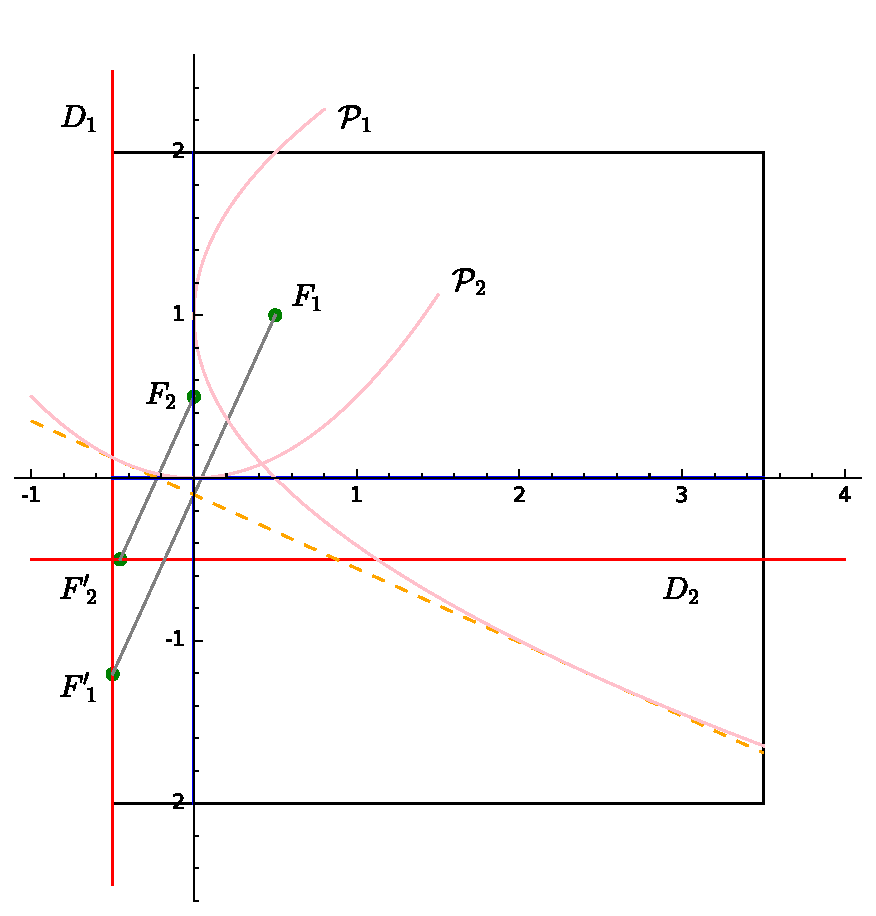
\includegraphics [width=8cm,height=8cm] {cubic_equation.pdf}
\end{center}
\end{figure}

\item[(a)] By Exercise 7, the focus and directrix of ${\mathscr P} _1 : (y-1)^2 = 2x$ are $$F_1\left (\frac{1}{2},1\right), \qquad D_1 : x = -\frac{1}{2},$$
and the focus and directrix of ${\mathscr P} _2 : y = \frac{x^2}{2}$ are $$F_2\left(0,\frac{1}{2}\right), \qquad D_2 : y = -\frac{1}{2}.$$

As all the points have rational coordinates, and the lines rational coefficients, they are constructible by origami. More precisely, take two arbitrary points on the $x$-axis to represent $(0,0)$ and $(1,0)$. To respect the instructions, the directrix $D_1 : x = -1/2$ must be the left side of the sheet, so the $y$-axis is placed at $1/8$ of the length of the sheet, and the unit is $1/4$ of this length, so we obtain the $y$-axis by three vertical folds (see figure). 

To obtain the two foci $F_1,F_2$, and the directrix $D_2$, we divide in eight equal parts the sheet by horizontal folds.

\item[(b)] As seen in the preliminaries, the discriminant of $x^3+2x+1$ is $\Delta_f =  -59<0$, the equation (10.12) $m^3+am+b = 0$, where $a = 2,b=1$, has a unique real solution $\alpha$. As the slope of a common tangent to the parabolas ${\mathscr P} _1,{\mathscr P} _2$ is a  root of this equation, the slope of such a tangent is $m=\alpha$. Since the intersection point $M_1(x_1,y_1)$ of the tangent with the parabola ${\mathscr P} _1$ satisfies (10.10)
$$x_1 = \frac{b}{2m^2}, \qquad y_1 = \frac{b}{m} + \frac{a}{2}$$
this intersection point is determined by $m = \alpha$, and similarly the tangent point  $M_2(x_2,y_2)$ with ${\mathscr P} _2$ is uniquely determined by 
$$x_2 = m, \qquad y_2 = \frac{m^2}{2},$$ so there is at most one common tangent to the two parabolas, and at most one way to take the focus of each parabola to a point on the corresponding directrix.

Conversely, we must prove the existence of a common tangent.

Let $D$ the line of slope $\alpha$ passing by $M_2(x_2,y_2)$, with $(x_2,y_2) = (\alpha,\frac{\alpha^2}{2})$. The equation of $D$ is given by $y-\frac{\alpha^2}{2} = \alpha (x-\alpha)$, so
$$D : -\alpha x + y +\frac{\alpha^2}{2}.$$

$D$ contains $M_1(x_1,y_1)$, where $(x_1,y_1) = (\frac{1}{2\alpha^2},1+\frac{1}{\alpha})$, since
$$-\alpha\left (\frac{1}{2\alpha^2}\right) + 1 + \frac{1}{\alpha} + \frac{\alpha^2}{2} = \frac{1}{2\alpha}(\alpha^3+2\alpha+1) = 0.$$

By Example 10.3.2 and Exercise 4, the slope of the tangent $T_1$ to ${\mathscr P} _1$ at $M_1$ is $m = \frac{b}{y_1-\frac{1}{2}a} = \alpha$, and the slope of the tangent $T_2$ to ${\mathscr P} _2$ at $M_2$ is $m = x_2 = \alpha$, so $D = T_1 = T_2$, therefore $D$ is tangent to ${\mathscr P} _1$ and ${\mathscr P} _2$. This proves the existence of one common tangent $D$ to the two parabolas, with equation
$$D : -\alpha x + y +\frac{\alpha^2}{2}.$$

Conclusion: there is exactly one way to take the focus of each parabola to a point on the corresponding directrix.

To obtain the corresponding line (the dotted line of the figure) by an origami fold, we take $F_1$ to $D_1$ (the left side of the sheet), and simultaneously $F_2$ to $D_2$. The slope $m$ of this line is the root $\alpha$ of $x^3 + 2x +1$.


\item[(c)] Let $F'_2$ be the reflexion of the focus $F_2$ of ${\mathscr P} _2$ about the common tangent $D$, and $M_2$ the point of tangency. By Exercise 3, the line $(M_2F'_2)$ is parallel to the $y$-axis, so by (10.11) the abscissa of $F'_2$ is $$x_2 =m.$$
 The intersection of the vertical fold  passing by $F'_2$ with the $x$-axis gives the point $(m,0)$, with $m\approx -0.45$. 
 
 We have resolved the equation $x^3 + 2x + 1 = 0$ by origami !
 
\end{proof}

\paragraph{Ex. 10.3.6}

{\it Suppose that in the situation of C3, we have points $\alpha_1\ne \alpha_2$ not lying on lines $l_1\ne l_2$. Also assume that $l_1$ and $l_2$ are parallel and that there is a line $l$ satisfying C3 (i.e., $l$ reflects $\alpha_i$ to a point of $l_i$ for $i=1,2$). Prove that the distance between $l_1$ and $l_2$ is at most the distance between $\alpha_1$ and $\alpha_2$. This makes it easy to find examples where the line described in C3 does not exist.
}

\begin{figure}[htbp]
\begin{center}
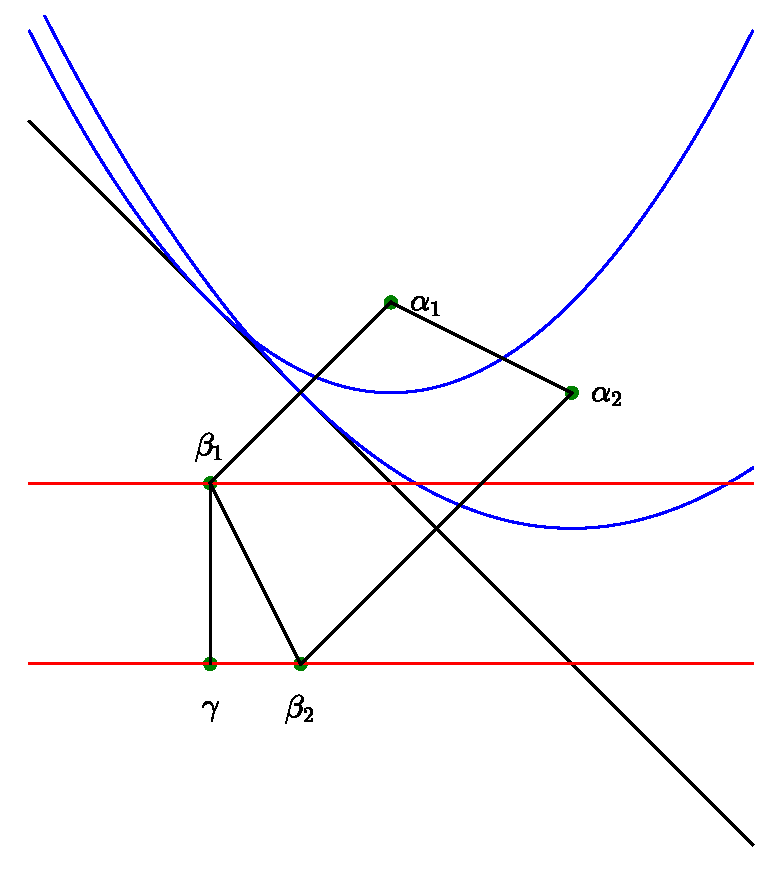
\includegraphics [width=7cm,height=7.5cm]  {parabolas0.pdf}
\end{center}
\end{figure}

\begin{proof}
Suppose that $l$ reflects $\alpha_1$ to $\beta_1 \in l_1$ and $\alpha_2$ to $\beta_2 \in l_2$.

Let $d =d(l_1,l_2)$ the distance between $l_1$ and $l_2$. If $\gamma$ is the orthogonal projection of $\beta_1$ on $l_2$, then by definition, $d = |\beta_1 - \gamma|$. By Pythagoras Theorem,
$$|\beta_1 - \gamma|^2 + |\gamma - \beta_2|^2 = |\beta_1 - \beta_2|^2.$$
Therefore $d^2 = |\beta_1 - \gamma|^2 \leq |\beta_1 - \beta_2|^2$, so $$d \leq |\beta_1 - \beta_2|.$$
Moreover the the reflexion about $l$ preserves the distances between points, so
$$|\beta_1 - \beta_2| = |\alpha_1 - \alpha_2|.$$

To conclude, the distance $d$ between $l_1$ and $l_2$ is at most the distance between $\alpha_1$ and $\alpha_2$.

For instance, let $l_1$ be the line with equation $y=0$, $l_2$ with equation $y=-2$, $\alpha_1 = i, \alpha_2 = 1+i$. Then $d = d(l_1,l_2) = 2 > |\alpha_1 - \alpha_2 |$, so there is no line $l$ that reflects $\alpha_1$ on a point on $l_1$ and $\alpha_2$ on a point on $l_2$. In other words, there is no common tangent to the two parabolas with focus $\alpha_i$ and directrix $l_i$, $i=1,2$, with equations
\begin{align*}
{\mathscr P} _1 &: y = \frac{1}{2} (x^2+1)\\
{\mathscr P} _2 &: y = \frac{1}{6} (x^2 - 2x-2)
\end{align*}
(see figure).
\begin{figure}[htbp]
\begin{center}
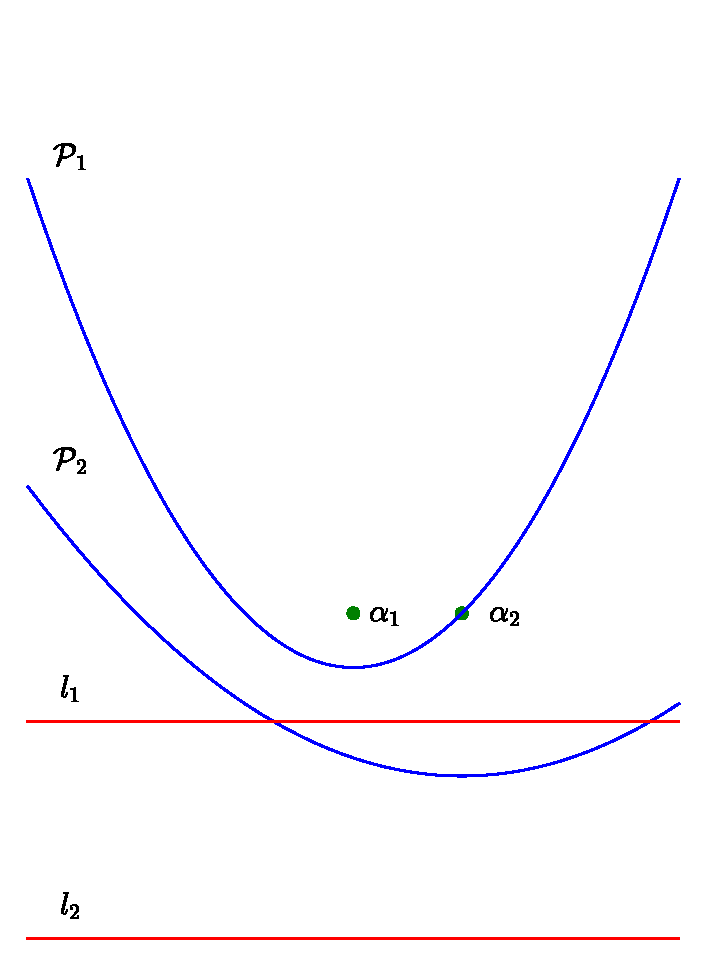
\includegraphics[width=5cm, height=6cm]  {parabolas.pdf}
\end{center}
\end{figure}
\end{proof}


\paragraph{Ex. 10.3.7}

{\it Consider the parabolas $\left (y-\frac{1}{2}a\right)^2 = 2bx$ and $y = \frac{1}{2} x^2$ from (10.9).
\be
\item[(a)] Show that the first parabola has focus $\left(\frac{1}{2}b,\frac{1}{2}a\right)$ and directrix $x=-\frac{1}{2} b$.
\item[(b)] Show that the second parabola has focus $\left(0,\frac{1}{2}\right)$ and directrix $y=-\frac{1}{2}$.
\ee
Hence the focus and directrix of the first parabola are defined over any subfield of $\R$ containing $a$ and $b$. For the second, this is true over any subfield of $\R$.
}

\begin{proof}
\item[(a)]
Let ${\mathscr P} _1$ the parabola with focus $F\left(\frac{1}{2}b,\frac{1}{2}a\right)$ and directrix $D : x=-\frac{1}{2} b$. Let $M(x,y)$ a point of the plane and $H(-\frac{1}{2}b,y)$ the orthogonal projection of $M$ on $D$. Then
\begin{align*}
M(x,y) \in {\mathscr P} _1 &\iff MF^2 = MH^2\\
& \iff \left(x-\frac{b}{2}\right)^2 + \left ( y -\frac{a}{2} \right)^2 = \left(x+\frac{b}{2}\right)^2\\
&\iff  \left ( y -\frac{a}{2} \right)^2 = 2bx.
\end{align*}
So the first parabola $\left (y-\frac{1}{2}a\right)^2 = 2bx$ has focus $\left(\frac{1}{2}b,\frac{1}{2}a\right)$ and directrix $x=-\frac{1}{2} b$.

\item[(b)] Let ${\mathscr P} _2$ the parabola with focus $F\left(0,\frac{1}{2}\right)$ and directrix $D : x=-\frac{1}{2} $. Let $M(x,y)$ a point of the plane and $H(0,-\frac{1}{2})$ the orthogonal projection of $M$ on $D$. Then
\begin{align*}
M(x,y) \in {\mathscr P} _2 &\iff MF^2 = MH^2\\
& \iff x^2 + \left ( y -\frac{1}{2} \right)^2 = \left(y+\frac{1}{2}\right)^2\\
&\iff x^2 = 2y.
\end{align*}
So the second parabola $y = x^2/2$ has focus $\left(0,\frac{1}{2}\right)$ and directrix $y=-\frac{1}{2}$.
\end{proof}

\paragraph{Ex. 10.3.8}

{\it Complete the proof of Theorem 10.3.6 sketched in the text.

\bigskip

{\bf Theorem 10.3.6} Let $\alpha \in \C$  be algebraic over $\Q$ and let $\Q \subset L$ be the splitting field of the minimal polynomial of $\alpha$ over $\Q$. Then $\alpha$ is an origami number if and only if $[L:\Q] = 2^a3^b$ for some integer $a,b\geq 0$.
}

\begin{proof} 

We first prove that $\Q \subset \cal O$ is a normal extension. 
Let $\alpha \in {\cal O}$, and let $f(x)$ be the minimal polynomial of $\alpha$ over $\Q$. By Theorem 10.3.4, there are subfields
$$\Q=F_0\subset F_1\subset \cdots \subset F_{n-1} \subset F_n \subset \C$$
such that $\alpha \in F_n$ and $[F_i:F_{i-1}] = 2$ or $3$ for $1\leq i \leq n$.

By Exercise 10.1.7, there exists a Galois closure $\Q\subset M$ of $\Q\subset F$ such that $M\subset \C$, so $\Q \subset F_n \subset M \subset \C$ and $\Q \subset M$ is a Galois extension.
Note that $f$ splits completely in $M$, since $M$ is normal over $\Q$, $f$ is irreducible over $\Q$, and $\alpha \in F_n \subset M$ is a root of $f$.

Now let $\beta \in M$ be any root of $f$. By Proposition 5.1.8, there is $\sigma \in \Gal(M/\Q)$ such that $\sigma(\alpha) = \beta$. Applying $\sigma$ to the fields $\Q=F_0 \subset \cdots \subset F_n \subset M$ gives
$$\Q \subset \sigma(\Q)=\sigma(F_0) \subset \cdots \subset \sigma(F_n)$$
such that $[\sigma(F_i):\sigma(F_{i-1}] = [F_i:F_{i-1}] = 2$ or $3$ for all $i$.

By Theorem 10.3.4, $\beta = \sigma(\alpha) \in \sigma(F_n)$ is an origami number, so $\beta \in {\cal O}$, so we can conclude that $ \Q \subset \cal O$ is a normal extension.
\be
\item[$\bullet$] Suppose that $\alpha \in {\cal O}$  and let $\Q \subset L$ be the splitting field of the minimal polynomial $f$ of $\alpha$ over $\Q$. Since $\Q \subset \cal O$ is normal, $L \subset {\cal O}$. By the theorem of the Primitive Element, we have $L = \Q(\gamma)$ for some $\gamma \in L$. Since $\gamma \in {\cal O}$, there are subfields
$$\Q=F'_0\subset F'_1\subset \cdots \subset F'_{n-1} \subset F'_m \subset \C$$
such that $\gamma \in F'_m$ and $[F'_i:F'_{i-1}] = 2$ or $3$ for $1\leq i \leq m$.

As $\Q \subset \Q(\gamma) \subset F'_m$, by the Tower Theorem, 

$[L : \Q] = [\Q(\gamma) : \Q]$ divides $[F'm:\Q] = 2^u3^v,\ u,v \in \N$, so 
\begin{center}
$[L:\Q] = 2^a3^b$ for some integer $a,b\geq 0$.
\end{center}

\item[$\bullet$] Conversely, suppose that $[L:\Q] = 2^a3^b$ for some integer $a,b\geq 0$.

Since $\Q \subset L$ is Galois, then $G =\Gal(L/\Q)$ satisfies $|G | = [L:\Q]$ is of the form
$$|G| = 2^a 3^b.$$
By Burnside's $p^nq^m$ Theorem (Theorem 8.1.8), $G$ is solvable, so we have subgroups
$$\{e\}=G_m \subset G_{m-1} \subset \cdots \subset G_1 \subset G_0 = G = \Gal(L/\Q)$$
such that $G_i$ is normal in $G_{i-1}$ of index 2 or 3, since $|G| = 2^a 3^b$. The Galois Correspondence Theorem gives
$$\Q=L_{G_0} \subset L_{G_1} \subset \cdots \subset L_{G_m} = L,$$
where $[L_{G_i}:L_{G_{i-1}}] = 2$ or 3 for all $i$.

By Theorem 10.3.4, $\alpha \in L$ is an origami number.
\ee
\end{proof}

\paragraph{Ex. 10.3.9}

{\it Prove Corollary 10.3.9.

\bigskip

{\bf Corollary 10.3.9} Let $f(x) \in \Q[x]$ be a polynomial of degree $\leq 4$. Then the roots of $f(x)$ are origami numbers, i.e, we can solve $f(x) = 0$ by origami.
}

\begin{proof} Let $\alpha$ be a root of $f(x)$, with $d = \deg(f) \leq 4$. 

Let $L$ be the splitting field of $\alpha$. 

Recall that the Galois group $\Gal(L/\Q)$ is isomorphic to a subgroup of $S_4$, so 
$$ |\Gal(L/\Q)| = [L:\Q]\ \mathrm{divides} \  4!.$$
So $[L:\Q]$ divides $4! = 2^3 \times 3$ , therefore $[L:\Q] = 2^a 3^b$ for some $a,b$ with  $0\leq a \leq 3,\  0 \leq b \leq 1$. By Theorem 10.3.6 and Exercise 8, $\alpha$ is an origami number.

\end{proof}

\paragraph{Ex. 10.3.10}

{\it In Example 10.3.10, prove that $l$ meets $l_1$ and $l_2$ at the points $Q_1$ and $Q_2$ given in (10.13) and (10.14). Also draw the four lines whose slopes are the roots of (10.15).
}
\begin{figure}[htbp]
\begin{center}
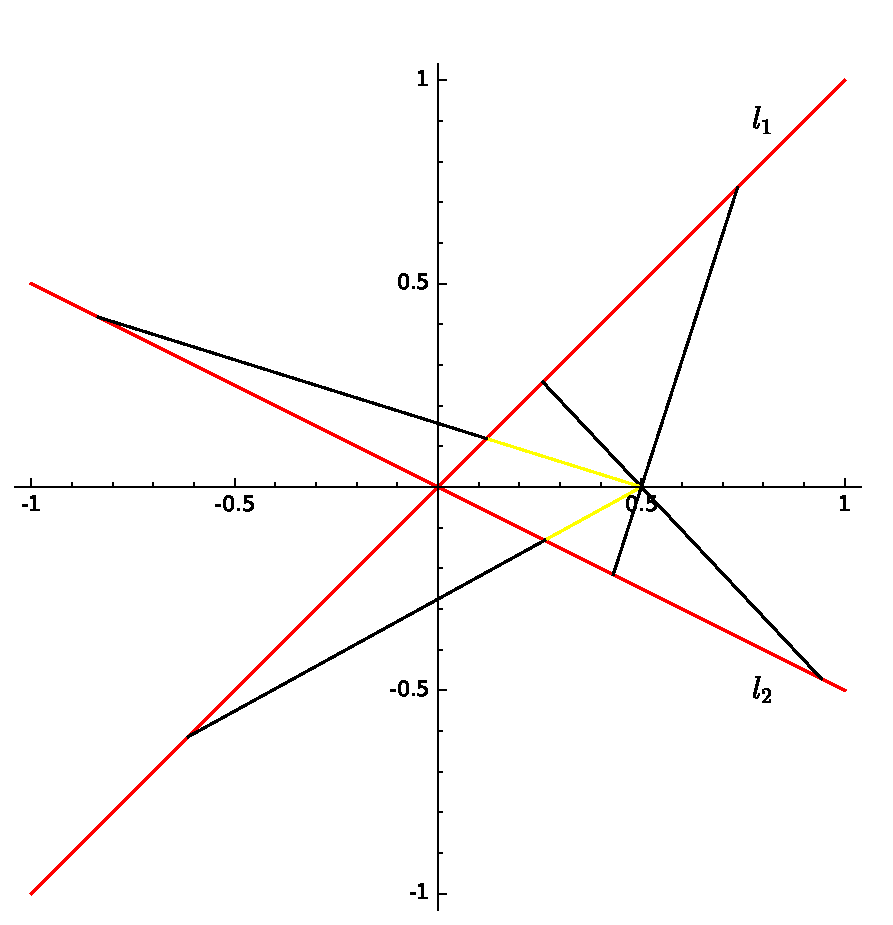
\includegraphics [width=8cm,height=8cm] {marquedRulers.pdf}
\end{center}
\end{figure}

\begin{proof}
The equation of the line $l$ with slope $m$ through $P=(\frac{1}{2},0)$ is
$$ l: y = m\left (x-\frac{1}{2}\right).$$

The intersection point $(x_1,y_1)$ of $l$ with $l_1: y=x$ is given by the system
\begin{align*}
y_1 &= x_1,\\
y_1 &= m\left (x_1-\frac{1}{2}\right),
\end{align*}
which gives $x_1 = m\left (x_1-\frac{1}{2}\right)$,  $2x_1 = 2mx_1-m$, so
$$Q_1 = (x_1,y_1) = \left ( \frac{m}{2m-2}, \frac{m}{2m-2}\right).$$
The intersection point $(x_2,y_2)$ of $l$ with $l_2: y=-\frac{1}{2}x$ is given by the system
\begin{align*}
y_2 &= -\frac{1}{2}x_2,\\
y_2 &= m\left (x_2-\frac{1}{2}\right),
\end{align*}
which gives $-\frac{1}{2}x_2 = m\left (x_2-\frac{1}{2}\right)$, so
$$Q_2 = (x_2,y_2) = \left ( \frac{m}{2m+1}, -\frac{m}{2(2m-2)}\right).$$
Therefore
\begin{align*}
Q_1Q_2 = 1 &\iff 1 = (x_2-x_1)^2 + (y_2-y_1)^2 \\
&\iff 1 = \left(\frac{m}{2m+1} -  \frac{m}{2m-2}\right)^2 + \left(-\frac{m}{2(2m+1)} - \frac{m}{2m-2}\right)^2 \\
&\iff 1 = m^2 \left[\left(\frac{2}{4m+2} - \frac{1}{2m-2}\right)^2 + \left(\frac{1}{4m+2} + \frac{1}{2m-2}\right)^2 \right]\\
& \iff 1 = \frac{m^2}{(4m+2)^2(2m-2)^2} \left\{ [(2(2m-2)-(4m+2)]^2 + [2m-2+4m+2]^2\right \}\\
&\iff (4m+2)^2(2m-2)^2 = m^2(36+36m^2)\\
&\iff 16 (2m+1)^2(m-1)^2 = 36 m^2(1+m^2)\\
&\iff 4(2m+1)^2(m-1)^2 = 9 m^2(1+m^2)\\
&\iff 16 m^4-16m^3-12m^2+8m+ 4 = 9 m^4 + 9m^2\\
&\iff 7m^4-15m^3-21m^2+8m+4 = 0.
\end{align*}

We obtain the four slopes and the figure with the following SAGE instructions:
\begin{verbatim}
m = var('m')
p = 7*m^4-16*m^3-21*m^2+8*m+4
l = solve(p,m)
sols = [eq.right() for eq in l]
slopes = [sol.n() for sol in sols]; slopes

		[-1.06517627861170, -0.312773186089791, 0.551041848035361, 3.11262190238042]
 

P = (1/2,0)
g = plot(x,x,xmin,xmax,color = 'red')
g += plot(-1/2*x,x,xmin,xmax, color = 'red')
for m in slopes:
    x1,x2 = m/(2*m-2),m/(2*m+1)
    Q1,Q2 = (x1,x1),(x2,-1/2*x2)
    g += line([Q1,P], color = 'yellow')
    g += line([Q1,Q2], color = 'black')
    
texte1 = text("$l_1$",(0.8,0.9), fontsize=15, rgbcolor=(0,0,0))
texte2 = text("$l_2$",(0.8,-0.5), fontsize=15, rgbcolor=(0,0,0))
g += texte1 + texte2
g.show(aspect_ratio=1)
g.save('marquedRulers.pdf',aspect_ratio=1,xmin=-1,xmax=1,ymin=-1,ymax=1)
\end{verbatim}
\end{proof}

\paragraph{Ex. 10.3.11}

{\it This exercise will give an example of a cubic equation that arises from verging. Consider the lines $l_1$ defined by $y=0$ and $l_2$ defined by $y=x$ and verge from $P = (1,\frac{1}{2})$ using a marked ruler. Show that this gives the vertical line $x=1$ together with three nonvertical lines whose slopes $m$ satisfy the cubic equation
$$ 4m^3+m^2-4m+1 = 0.$$
Also show that the nonvertical lines cannot be constructed by straightedge and compass.
}

\begin{figure}[htbp]
\begin{center}
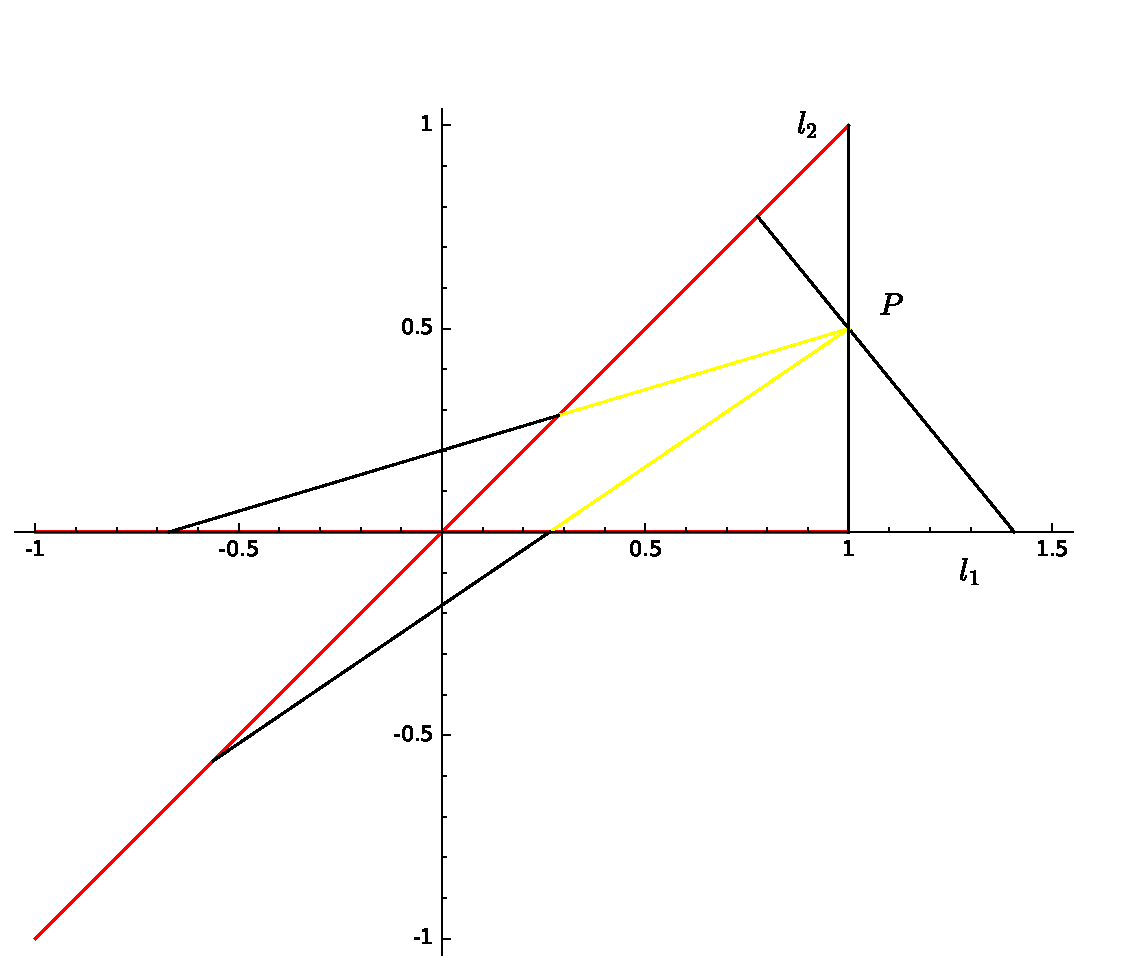
\includegraphics [width=9cm,height=8cm] {marquedRulers3.pdf}
\end{center}
\end{figure}
\begin{proof}
Here a solution is the vertical line $x = 1$, corresponding to $m = \infty$, since the intersection of this line with $l_1$ and $l_2$ are the points $Q_1=(1,0), Q_2 = (1,1)$ such that $Q_1Q_2 = 1$.

Any nonvertical line $l$ with slope $m$ through $P = (1,\frac{1}{2})$ has an equation
$$l : y - \frac{1}{2} = m (x-1).$$
The intersection point of $l$ with $l_1 : y = 0$ and the intersection of $l$ with $l_2 : y=x$ are the points
\begin{align*}
Q_1 &= (x_1,y_1) =  \left (\frac{2m-1}{2m},0 \right),\\
Q_2 &= (x_2,y_2) =  \left (\frac{2m-1}{2m-2}, \frac{2m-1}{2m-2} \right).
\end{align*}
Therefore
\begin{align*}
Q_1Q_2 = 1 &\iff1= (x_2-x_1)^2 + (y_2-y_1)^2\\
&\iff 1=\left(\frac{2m-1}{2m-2} - \frac{2m-1}{2m} \right)^2 + \left(\frac{2m-1}{2m-2} \right)^2\\
&\iff (2m-1)^2 \left[ \left(\frac{2}{2m(2m-2)} \right)^2 + \frac{1}{(2m-2)^2} \right]\\
&\iff 1 = \frac{(2m-1)^2}{(2m-2)^2} \left ( \frac{1}{m^2} + 1 \right)\\
&\iff 4m^2(m-1)^2 = (2m-1)^2(m^2 + 1)\\
&\iff 4m^4 - 8m^3 + 4m^2 = 4 m^4 - 4m^3+ 5m^2 - 4m+1\\
&\iff 4m^3+m^2 - 4m+1 = 0.
\end{align*}
Let $f(x) = 4x^3+x^2-4x+1$, then 
$$\lim_{x \to -\infty}f(x) = -\infty,\quad  f\left(-\frac{2}{3}\right) = \frac{79}{27} >0,\quad  f\left(\frac{1}{2}\right) = -\frac{1}{4}<0,\quad  \lim_{x \to +\infty} f(x)= +\infty.$$ Therefore $f(x)$ has three real roots
$$m_1 \approx 0.2991, m_2 \approx -1.2290, m_3 \approx 0.6799.$$
This gives 4 solutions with $m=\infty$.
(see figure.)

$f(x)$ has no rational root. Indeed , if $\alpha = \frac{p}{q}, p,q \in \Z, q>0, p\wedge q = 1$ is a root of $f$, then $4p^3+p^2q-4pq^2+q^3 = 0$, so $p^3 \mid 1, q^3 \mid 2$, therefore $p = \pm 1, q =1$, so $\alpha = \pm 1$, but neither 1 nor $-1$ is a root of $f$. Since $\deg(f) = 3$, $f$ is irreducible over $\Q$ and the minimal polynomial of $m_1,m_2$ or $m_3$ over $\Q$ is $f$.

Let $L = \Q(m_1,m_2,m_3)$ the splitting field of $f$.
The discriminant of $f$ is $\Delta_f = 316 = 2^2 \times 79$, where $79$ is prime, so $\Delta_f$ is not a square in $\Q$, so $\Gal(L:\Q) \simeq S_3$, therefore $[L:\Q] = 6$ is not a power of 2, so $m_1,m_2,m_3$ are not constructible numbers. Therefore the nonvertical lines are not constructible by straightedge and compass.
\end{proof}

\paragraph{Ex. 10.3.12}

{\it Prove that $\angle PRO = \theta/3$ in the construction (10.18). 
}

\begin{proof} 
 Let $\alpha = \angle PRO$. Since $QR = QO=1$ , $\triangle QRO$ is isosceles, so $\angle QOR = \alpha$. Therefore the extern angle $\angle OQP = 2\alpha$. Since $OQ = OP =1$, $\triangle OPQ$ is isosceles, so 
 $$\angle OQP = \angle OPQ = 2\alpha.$$
 Therefore $\angle QOP = \pi - 4\alpha$. Since $\angle ROQ + \angle QOP + \theta = \pi,$ $\alpha + (\pi - 4 \alpha) + \theta = \pi$, so $\theta = 3\alpha$,
 $$\angle PRO = \frac{\theta}{3}.$$
\end{proof}


\paragraph{Ex. 10.3.13}

{\it According to [15] (G.E.Martin, Geometric Constructions), Pappus used a marked ruler to trisect angles as follows. Given an angle $0<\theta < \pi/2$, write it as $\theta = \angle POA$, where:
\be
\item[$\bullet$] The distance between $P$ and $O$ is $1/2$.
\item[$\bullet$] The line $l_1$ determined by $P$ and $A$ is perpendicular to the line determined by $O$ and $A$.
\ee
Any angle $0 < \theta < \pi/2$ can be put in this form by a marked-ruler construction. Finally, let $l_2$ be the line through $P$ that is perpendicular to $l_1$. Then verging with $O$ and the lines $l_1$ and $l_2$ gives points $Q \in l_1$ and $R \in l_2$ such that $Q$ and $R$ are one unit apart.

Prove that $\angle QOA = \theta/3$.
}
\begin{figure}[htbp]
\begin{center}
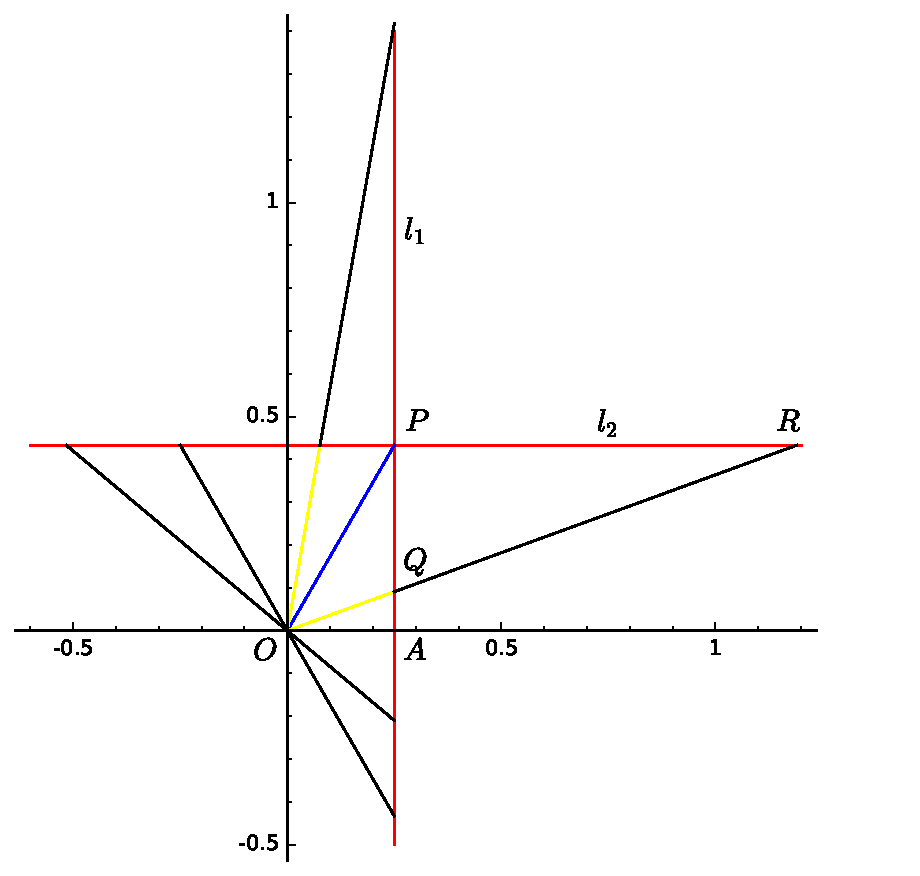
\includegraphics[width=10.8cm,height=11.4cm]{markedRulers5.pdf}
\end{center}
\end{figure}

\begin{proof}
As $OP = \frac{1}{2}$, $P = \left(\frac{1}{2} \cos \theta, \frac{1}{2} \sin \theta \right)$, and $A = \left(\frac{1}{2} \cos \theta,0 \right)$. The vertical line is not a solution. The equation of every nonvertical line  $l$ with slope $m$ passing through $Q$ is $$l : y = mx,$$ where $m = \tan \alpha$ and $\alpha\in ] -\frac{\pi}{2}, \frac{\pi}{2}[$ is a measure of $\angle AOR$.
The equations of $l_1,l_2$ are 
\begin{align*}
l_1  &: x = \frac{1}{2} \cos \theta,\\
l_2 &: y = \frac{1}{2} \sin \theta.
\end{align*}
The intersection point $Q = (x_1,y_1)$ of $l$ with $l_1$ is given by
\begin{align*}
x_1 &= \frac{1}{2} \cos \theta,\\
y_1 &= m \frac{1}{2} \cos \theta,
\end{align*}
and the intersection point $R$ of $l$ with $l_2$ is given by
\begin{align*}
x_2 &= \frac{1}{2m} \sin \theta,\\
y_2 & = \frac{1}{2} \sin \theta.
\end{align*}
Therefore
\begin{align*}
QR = 1 &\iff 1 = (x_2-x_1)^2 + (y_2-y_1)^2\\
&\iff 1 = \left ( \frac{1}{2m} \sin \theta -  \frac{1}{2} \cos \theta \right)^2 + \left( \frac{1}{2} \sin \theta - m \frac{1}{2} \cos \theta\right)^2\\
&\iff 1 = \frac{1}{4m^2} (\sin \theta - m \cos \theta)^2 + \frac{1}{4} (\sin \theta - m \cos \theta)^2\\
&\iff 4 m^2  = (\sin \theta - m \cos \theta)^2(m^2+1)\\
&\iff 0 = \left (\sin \theta - m \cos \theta - \frac{2m}{\sqrt{m^2+1}}\right )\left (\sin \theta - m \cos \theta + \frac{2m}{\sqrt{m^2+1}}\right).
\end{align*}
Note that, since $m = \tan \alpha$,
$$ \frac{2m}{\sqrt{m^2+1}} = \frac{2 \, \frac{\sin \alpha}{\cos \alpha}} {\sqrt{\frac{\sin^2 \alpha}{\cos^2 \alpha} + 1}}  = 2 \sin \alpha.$$
Moreover 
$$\sin \theta - m \cos \theta = \sin \theta - \frac{\sin \alpha}{\cos \alpha} \cos \theta = \frac{\sin(\theta - \alpha)}{\cos \alpha}.$$
Therefore
\begin{align*}
 QR = 1 &\iff 0 = \left (\frac{\sin(\theta - \alpha)}{\cos \alpha} - 2 \sin \alpha \right) \left (\frac{\sin(\theta - \alpha)}{\cos \alpha} + 2 \sin \alpha \right)\\
 &\iff 0 = (\sin(\theta - \alpha) - \sin (2\alpha))(\sin(\theta - \alpha) + \sin (2\alpha))\\
 &\iff \sin(\theta - \alpha) =  \pm \sin (2\alpha)\\
 &\iff \theta -\alpha = 2 \alpha - k \pi  \quad \mathrm{or} \quad \theta - \alpha =  \pi - 2 \alpha + k \pi \qquad (k\in \Z)\\
 &\iff \alpha = \frac{\theta}{3} + k \frac{\pi}{3} \quad \mathrm{or} \quad \alpha = \pi - \theta + k \pi  \qquad (k \in \Z).
\end{align*}
Since $0 <\theta  < \frac{\pi}{2}$ and $-\frac{\pi}{2} < \alpha < \frac{\pi}{2}$, we obtain finally
$$QR = 1 \iff \alpha = \frac{\theta}{3} \quad \mathrm{or} \quad \alpha = \frac{\theta + \pi}{3}  \quad \mathrm{or} \quad \alpha = \frac{\theta - \pi}{3} \quad \mathrm{or} \quad  \alpha = -\theta .$$

The only solution $0 < \alpha < \theta$ is $\alpha = \theta/3$.

In the example of the angle $\theta = 60� = \pi/3$, where $\theta/3 = 20� = \pi/9$ is not constructible by straightedge and compass, we obtain $\alpha \in \left \{ \frac{\pi}{9}, \frac{4\pi}{9},-\frac{2\pi}{9}, - \frac{\pi}{3}\right \}$, all constructible with the marked ruler (see figure).
\end{proof}

{\bf Solution 2}
\begin{figure}[htbp]
\begin{center}
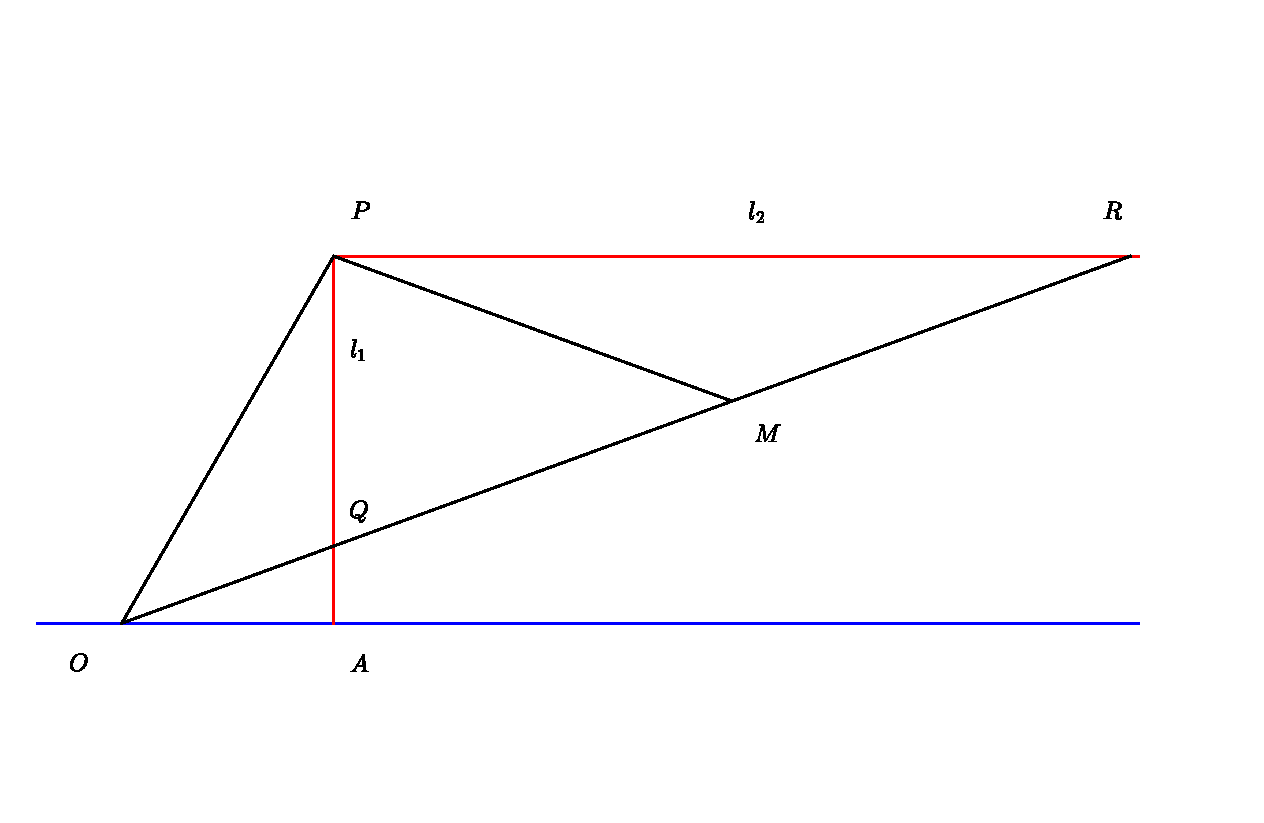
\includegraphics[width=7.8cm,height=5.4cm]{markedRulers6.pdf}
\end{center}
\end{figure}

\begin{proof}
We follow the indication of David A. Cox and give the more geometric proof of [15] (G.E.Martin, Geometric Constructions):

"Let $\angle AOR$ have measure $t$. Then $\angle PRO$ has measure $t$. Let $M$ be the midpoint of $Q$ and $R$. Since $\angle RPQ$ is right, then $P$ lies on the circle with diameter $\overline{RQ}$ by the converse of the Theorem of Thales. So $MQ = MP = MR = OP = 1/2$, and $\triangle MPR$ and $\triangle POM$ are isosceles triangles. Hence, $\angle MPR$ has measure $t$ by the Pons Asinorum, $\angle OMP$ has measure $2t$ by the Exterior Angle Theorem, and $\angle POM$ has measure $2t$ by the Pons Asinorum. Therefore, $\overrightarrow{OR}$ trisects $\angle POA$."
\end{proof}

\paragraph{Ex. 10.3.14}

{\it As explained in [21](C.R.Videla, {\it On points constructible from conics}), Pappus used intersections of conics to trisect angles as follows. Consider the unit circle centered at the origin, and let $0<\theta < \pi/2$. Then $P = (\cos \theta, \sin \theta)$ is the corresponding point on the unit circle. We assume that $P$ is known. Also let $O =(0,0)$ and set $A = (1,0)$. Thus $\theta = \angle POA$.
\be
\item[(a)] Consider the curve $C$ consisting of all points $Q = (x,y)$ such that the distance from $P$ to $Q$ is twice the distance from $Q$ to the $y$-axis. The curve $C$ intersects the unit circle at a point $R$ lying in the interior of $\angle POA$. Prove that $\angle ROA = \theta/3$.
\item[(b)] Show that the curve $C$ is a hyperbola. It follows that we have trisected an angle using the intersection of a hyperbola and a circle, i.e., an intersection of conics.
\ee
}

\begin{proof}
\be
\item[(a)]
Let $H$ the orthogonal projection of $R$ on the $x$-axis, and $S$ such that $H$ is the midpoint  of $RS$, so $S$ is the reflection of $R$ with regard to the $x$-axis. Since $R$ is on the curve $C$,
$$PR = 2 RA = RS,$$
therefore the measures of $\angle ROP$ and $\angle SOR$ are equal, and is twice the measure of $\angle AOR$, so $\overrightarrow{OR}$ trisects the angle $\angle POA$ and a measure of $\angle ROA$ is $\theta/3$.

\item[(b)] Let $Q=(x,y), H = (x,0), P = (\cos \theta, \sin \theta)$
\begin{align*}
Q \in C &\iff QP = 2 QH \iff QP^2 = 4 QH^2\\
&\iff(x- \cos \theta)^2 + (y-\sin \theta)^2 = 4 y^2\\
& \iff x^2 - 3 y^2  - 2 x \cos \theta  - 2 y \sin \theta +1 = 0.
\end{align*}
The discriminant of the quadratic form $a x^2 + bxy + cy^2 = x^2-3y^2$ is $\Delta = 12>0$, so $C$ is not empty and $C$ is a hyperbola.
\ee
\end{proof}

\paragraph{Ex. 10.3.15}

{\it In this exercise, we discuss a marked-ruler construction of cube roots due to Nicomedes and taken from [15]. Let $k$ be a real number such that $0<k<8$, and consider an isosceles triangle $\triangle ABC$ such that $AC$ and $BC$ have length 1 and AB has length $k/4$. Then extend $AC$ and $AB$ as indicated in the picture below, and choose $D$ on the extension of $AC$ so that $AD$ also has length 1. Finally, draw the line through $D$ and $B$.

Verging from $C$ with the lines $l_1$ and $l_2$ indicated above gives points $Q\in l_1$ and $R \in l_2$ that are one unit apart. Assume that $Q\ne D$.
\be
\item[(a)] Explain why the restriction $0<k<8$ is necessary.
\item[(b)] Prove that the distance between $B$ and $R$ is $\sqrt[3]{k}$.
\item[(c)] Explain how to give a marked-ruler construction for any $k>0$.
\ee
}

\begin{figure}[htbp]
\begin{center}
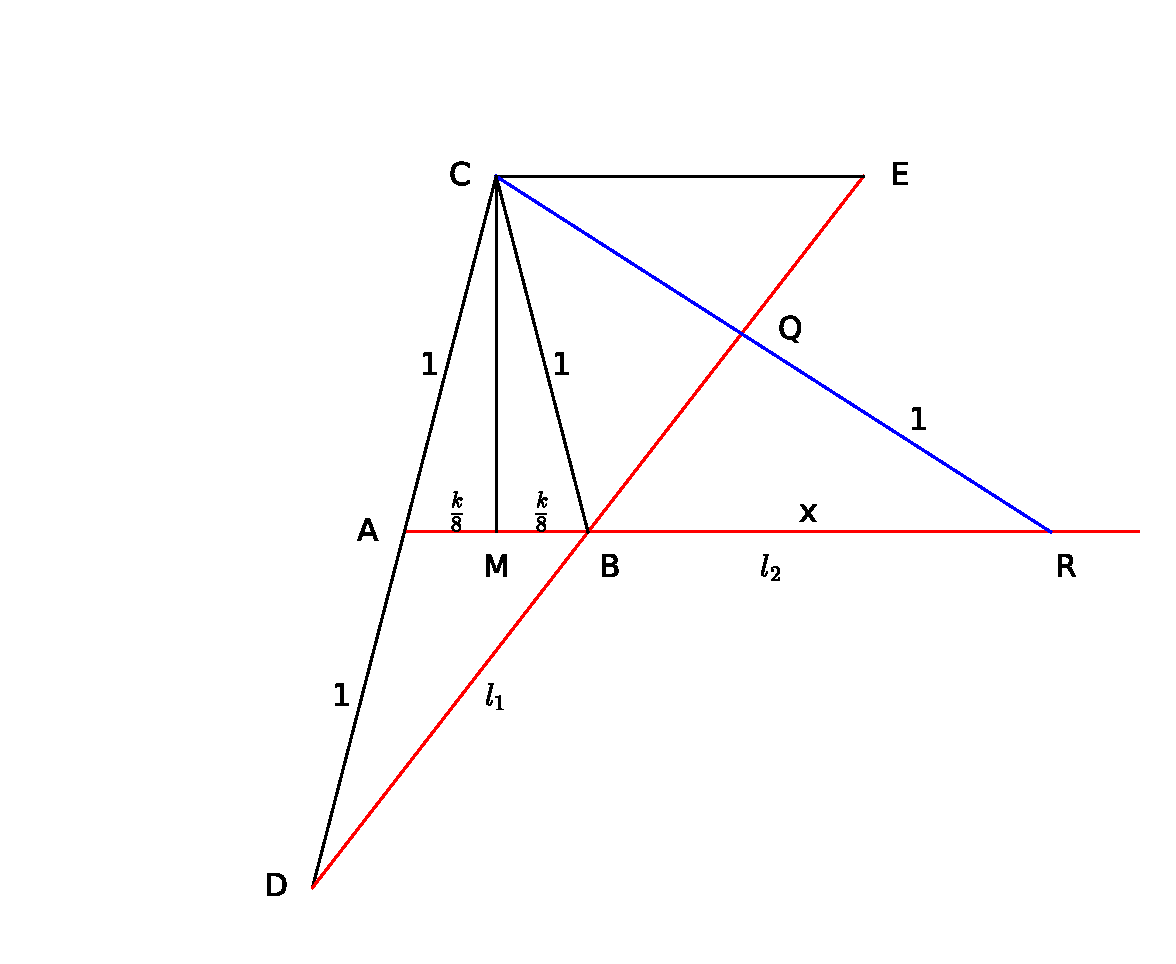
\includegraphics[width=12cm,height=8cm]{Nicomedes.pdf}
\end{center}
\end{figure}

\begin{proof}
\item[(a)] We suppose that $k\geq 0$. Let $I = M$ be the midpoint of $AB$. As $\triangle ABC$ is isosceles, by Pythagoras' Theorem, $CI^2 + (k/8)^2 = AC^2 = 1$,  therefore $0 \leq k/8\leq1$, so $k \leq 8$. If $k>8$, there exists no point $C$ with the conditions of the text. If $k=8$, $C$ is the midpoint of $AB$ and $l_1$ = $l_2$, and if $k=0$, $A=B$ and $l_2$ is not defined. The restriction $0<k<8$ is necessary.

\item[(b)] 2 solutions.

\be

	\item[{\bf Solution 1.}]  Personal solution with analytic geometry.
	
	Take the origin in $O = M$, where $M$ is the midpoint of $AB$, and take $MB,MC$ as the $x$ and $y$-axis. Write for simplicity $\lambda = MB = k/8, \mu = MC$, so $\lambda^2 + \mu^2 = 1$. The unknown is $x = \overline{BR}$.
	
	The coordinates of $A,B,C,D,R$ are
$$ A \left | 
\begin{array}{c}
  -\lambda\\
 0 
\end{array}
\right.
, \quad 
B \left | 
\begin{array}{c}
  \lambda\\
 0 
\end{array}
\right.
, \quad 
C \left | 
\begin{array}{c}
 0\\
\mu
\end{array}
\right.
, \quad 
D \left | 
\begin{array}{c}
  -2\lambda\\
-\mu
\end{array}
\right.
, \quad 
R \left | 
\begin{array}{c}
  \lambda + x\\
 0 
\end{array}
\right.
.
$$	
Let $(X,Y)$ any point in the plane.
\begin{align*}
(X,Y) \in l_1 = (DB) &\iff 0 = \begin{vmatrix} X - x_B & x_B - x_D \\Y-y_B & y_B - y_D \end{vmatrix} = \begin{vmatrix} X - \lambda & 3 \lambda \\Y&\mu \end{vmatrix}\\
	&\iff \mu(X-\lambda) - 3\lambda Y= 0.\\
\end{align*}
So the equation of $(DB)$ is
$$(DB) : \mu X - 3 \lambda Y = \lambda \mu.$$
Similarly,
\begin{align*}
(X,Y) \in (CR) &\iff 0 = \begin{vmatrix} X - x_C & -(x_R - x_C) \\Y-y_C &-(y_R-y_C) \end{vmatrix} = \begin{vmatrix} X  & -( \lambda +x)\\Y - \mu &\mu \end{vmatrix}\\
	&\iff \mu X +(\lambda+x) Y = \mu(\lambda + x) .\\
\end{align*}
So the equation of $(CR)$ is
$$(CR) : \mu X +(\lambda + x) Y =\mu(\lambda + x).$$

The coordinates $(x_Q,y_Q)$ are given by the system
\begin{align*}
\mu X - 3 \lambda Y &= \lambda \mu,\\
\mu X + (\lambda + x) Y &= \mu (\lambda +x).
\end{align*}
Since $\mu \ne 0$, this is equivalent to
\begin{align*}
(4\lambda + x) X &= 4\lambda(\lambda + x),\\
(4\lambda + x) Y &= \mu x,
\end{align*}
so
$$ Q\left | 
\begin{array}{c}
\frac{4 \lambda (\lambda + x)}{4\lambda +x}\\
\frac{\mu x}{4\lambda +x}
\end{array}
\right.
, \quad 
R \left | 
\begin{array}{c}
  \lambda + x\\
 0 
\end{array}
\right.
.
$$
Therefore 
\begin{align*}
QR = 1 &\iff 1 =  \left [ \frac{4 \lambda (\lambda + x)}{4\lambda +x} - (\lambda + x) \right ]^2 + \left [ \frac{\mu x}{4\lambda +x} \right]^2 \\
&\iff (4 \lambda + x)^2 = (\lambda + x)^2 x^2 + \mu^2 x^2\\
&\phantom{\iff (4 \lambda + x)^2\, } = x^4+ 2\lambda x^3 +( \lambda^2 + \mu ^2) x^2\\
&\phantom{\iff (4 \lambda + x)^2\, } = x^4 + 2 \lambda x^3 + x^2\\
&\iff x^4 + 2\lambda x^3 - 8 \lambda x - 16 \lambda^2 = 0\\
& \iff (x+ 2 \lambda)(x^3 - 8 \lambda) = 0\\
&\iff \left (x+ \frac{k}{4} \right)(x^3 - k)=0
\end{align*}

As $Q \ne D, R \ne A$, so $x \ne -k/4$. Therefore
$$QR = 1 \iff x = \sqrt[3]{k}.$$
Note: the factorization is easy because $x = -2 \lambda = -k/4$ gives the particular solution $R = A$.

The marked-ruler constructions of Pappus (for the trisection) and Nicomedes (for the cube root) give both a fourth degree equation with a known obvious solution.

	\item[{\bf Solution2.}]  From  [15] (G.E. Martin, Geometric Constructions):

" Let the parallel to $(AB)$ that passes through $C$ intersect $(DB)$ at $E$. So $\triangle ABD$ and $\triangle CDE$ are similar. Then, since $A$ bisects $CD$, we have $CE = 2 AB = k/2$. Also, since $\triangle QBR$ and $\triangle QCE$ are similar, we have $(k/2) / CQ = BR/1$. With $x = BR$, then $CQ = k/(2x)$. With $M$ the midpoint of $A$ and $B$, by two aplications of the Pythagorean Theorem, we now have
\begin{align*}
\left ( 1 + \frac{k}{2x} \right )^2 &= CR^2 = CM^2+MR^2 = (CA^2 - AM^2) + MR^2\\
&=1^2 - \left ( \frac{k}{8} \right)^2  + \left( x + \frac{k}{8}\right)^2
\end{align*}
(So, multiplying the two members by $8^2x^2$,
\begin{align*}
16(2x+k)^2 &= 8^2x^2 - k^2x^2 +x^2(8x+k)^2\\
64 x^2 + 64 kx + 16 k^2 &= 64 x^2 - k^2 x^2 + 64 x^4 + 16kx^3 + k^2 x^2\\
0 &= 64x^4 + 16kx^3 -64kx - 16k^2\\
0 &=4x^4 + kx^3 - 4kx -k^2. )
\end{align*}
Fortunately, this quartic easily factors as $(4x+k)(x^3-k) =0$. Since $4x+k>0$, then we must have $x^3 -k =0$. Therefore, $x$ is the real cube root of $k$, as desired."
\ee
\item[(c)]If $k$ is any positive number, let $s$ an integer such that $0 < k <2^{3s+3}$, so $0 < K <8$, where $K = \frac{k}{2^{3s}}$. The Nicomedes' construction applied to $K$ gives $\sqrt[3]{K}$, thus $\sqrt[3]{k} = 2^s \sqrt[3]{K}$ is constructible by marked-ruler.
\end{proof}

\paragraph{Ex. 10.3.16}

{\it Let $P$ be a point distance $b>0$ from a line $l$. Put a marked ruler though $P$ with one mark at $R \in l$. When $R$ moves along $l$, the other mark $Q_1$ or $Q_2$ (depending on which side of $l$ it is on) traces out the conchoid of Nicomedes.

We can relate the conchoid to constructions problems as follows.
\be
\item[(a)] Suppose we are given a point $P$ and lines $l_1,l_2$, and assume that $P \not \in l_1$. Prove that a point $Q$ is obtained by verging with $P$ and $l_1,l_2$ if and only if $Q$ is one of the points of intersection of $l_2$ with the conchoid determined by $P$ and $l_1$.
\item[(b)] Prove that the angle trisection of (10.18) can be interpreted as the intersection of the unit circle with the conchoid determined by $P$ and $l_1$.

\item[(c)] Suppose that $P = (0,0)$ and $l$ is the horizontal line $y=-b$. Prove that the polar equation of the conchoid is
$$r = b \csc \theta \pm 1,$$
where the minus sign gives the portion of the curve above $l$ and the plus sign gives the portion below.
\item[(d)] Under the assumptions of part (c), show that the Cartesian equation of the conchoid is
$$(x^2+y^2)(y-b)^2 = y^2.$$
By part (a), verging is the same as intersecting the conchoid with a line. Since the above equation has degree 4, this explains why verging leads to an equation of degree 4.
\ee
}

\begin{proof}
\be
\item[(a)] Let $Q \in l_2$. Then $Q$ is obtained by verging with $P$ and $l_1,l_2$ if and only if there is a point $R \in l_1$ such that $QR = 1$, if and only if $R$ is on the conchoid.

\item[(b)] As $QR=1$, with $R$ on $l$, $Q$ is on the conchoid determined by $P$ and $l$, and on the unit circle, so $Q$ is at the intersection of the unit circle and the conchoid.

\item[(c)] Here $P = (0,0)$ and $l$ is the horizontal line $y=-b, b>0$, in the Cartesian coordinates system $(P,\vec{e}_1,\vec{e}_2)$.   

If $R$ is any point on $l$, then $\overrightarrow{PR} = \rho  \vec{u}$, where 
$$\vec{u}  = \cos \theta \, \vec{e}_1 + \sin \theta\,  \vec{e}_2, \ \theta \in \R \setminus \{k \pi, k \in \Z\}.$$
The equation of the line $l_R = (PR)$ is given for $M =(x,y) \in l_R$ by $\det( \overrightarrow{PM}, \vec{u}) = 0$:
$$x \sin \theta - y \cos \theta=0,$$
thus $$ R = \left(-b\, \frac{\cos \theta}{\sin \theta}, -b\right).$$
Let $\mathscr{C} $ be the conchoid, and let $(r,\theta)$ the polar coordinates of a point $Q = (x,y) = (r \cos \theta, r \sin \theta)$ where $Q$ is a point in the line $PR$. Then 
$$\overrightarrow{PQ} = r \vec{u} = r (\cos \theta \, \vec{e}_1+ \sin \theta \, \vec{e}_2) ,$$
where $\theta \in \R \setminus \{k \pi, k \in \Z\}$, and $r \in \R$ may be positive or negative.
\begin{align*}
Q \in  \mathscr{C} & \iff  QR = 1\\
&\iff 1 =    \left(x + b\, \frac{\cos \theta}{\sin \theta} \right)^2 + (y + b)^2\\
&\iff \left ( r \cos \theta + b \frac{\cos \theta}{\sin \theta} \right)^2 + (r \sin \theta + b)^2 = 1\\
&\iff \left ( r + \frac{b}{\sin \theta} \right)^2 = 1\\
&\iff  r = \frac{-b}{\sin \theta}   \pm 1 \quad ( = -b \csc \theta \pm 1).
\end{align*}
 So the polar equation of the conchoid of Nicomedes is
  $$r = \frac{-b}{\sin \theta}   \pm 1, \theta \in \R \setminus \{k \pi, k \in \Z\},$$
where the sign of $\pm 1$ gives the two portions of the curve.  

$PR = \left | \frac{b}{\sin \theta} \right |$.

If $\theta \in ]0,\pi[$, then $r<0$ and $ -\frac{b}{\sin \theta}  < 0$,  so $\frac{-b}{\sin \theta} - 1$ give the portion below the line $l$, and  $\frac{-b}{\sin \theta} + 1$ give the portion above.   

If  $\theta \in ]-\pi,0[$, then $r>0$ and  $ -\frac{b}{\sin \theta}  > 0$, so $\frac{-b}{\sin \theta} - 1$ give the portion above the line $l$, and  $\frac{-b}{\sin \theta} + 1$ give the portion below.  

This is confirmed by the instruction "polar\_plot" with Sage, where the blue and red portions of the conchoid are exchanged when  $\theta \in ]0,\pi[$ and $\theta \in ]-\pi,0[$ (see figure).
 
\begin{figure}[htbp]
\begin{center}
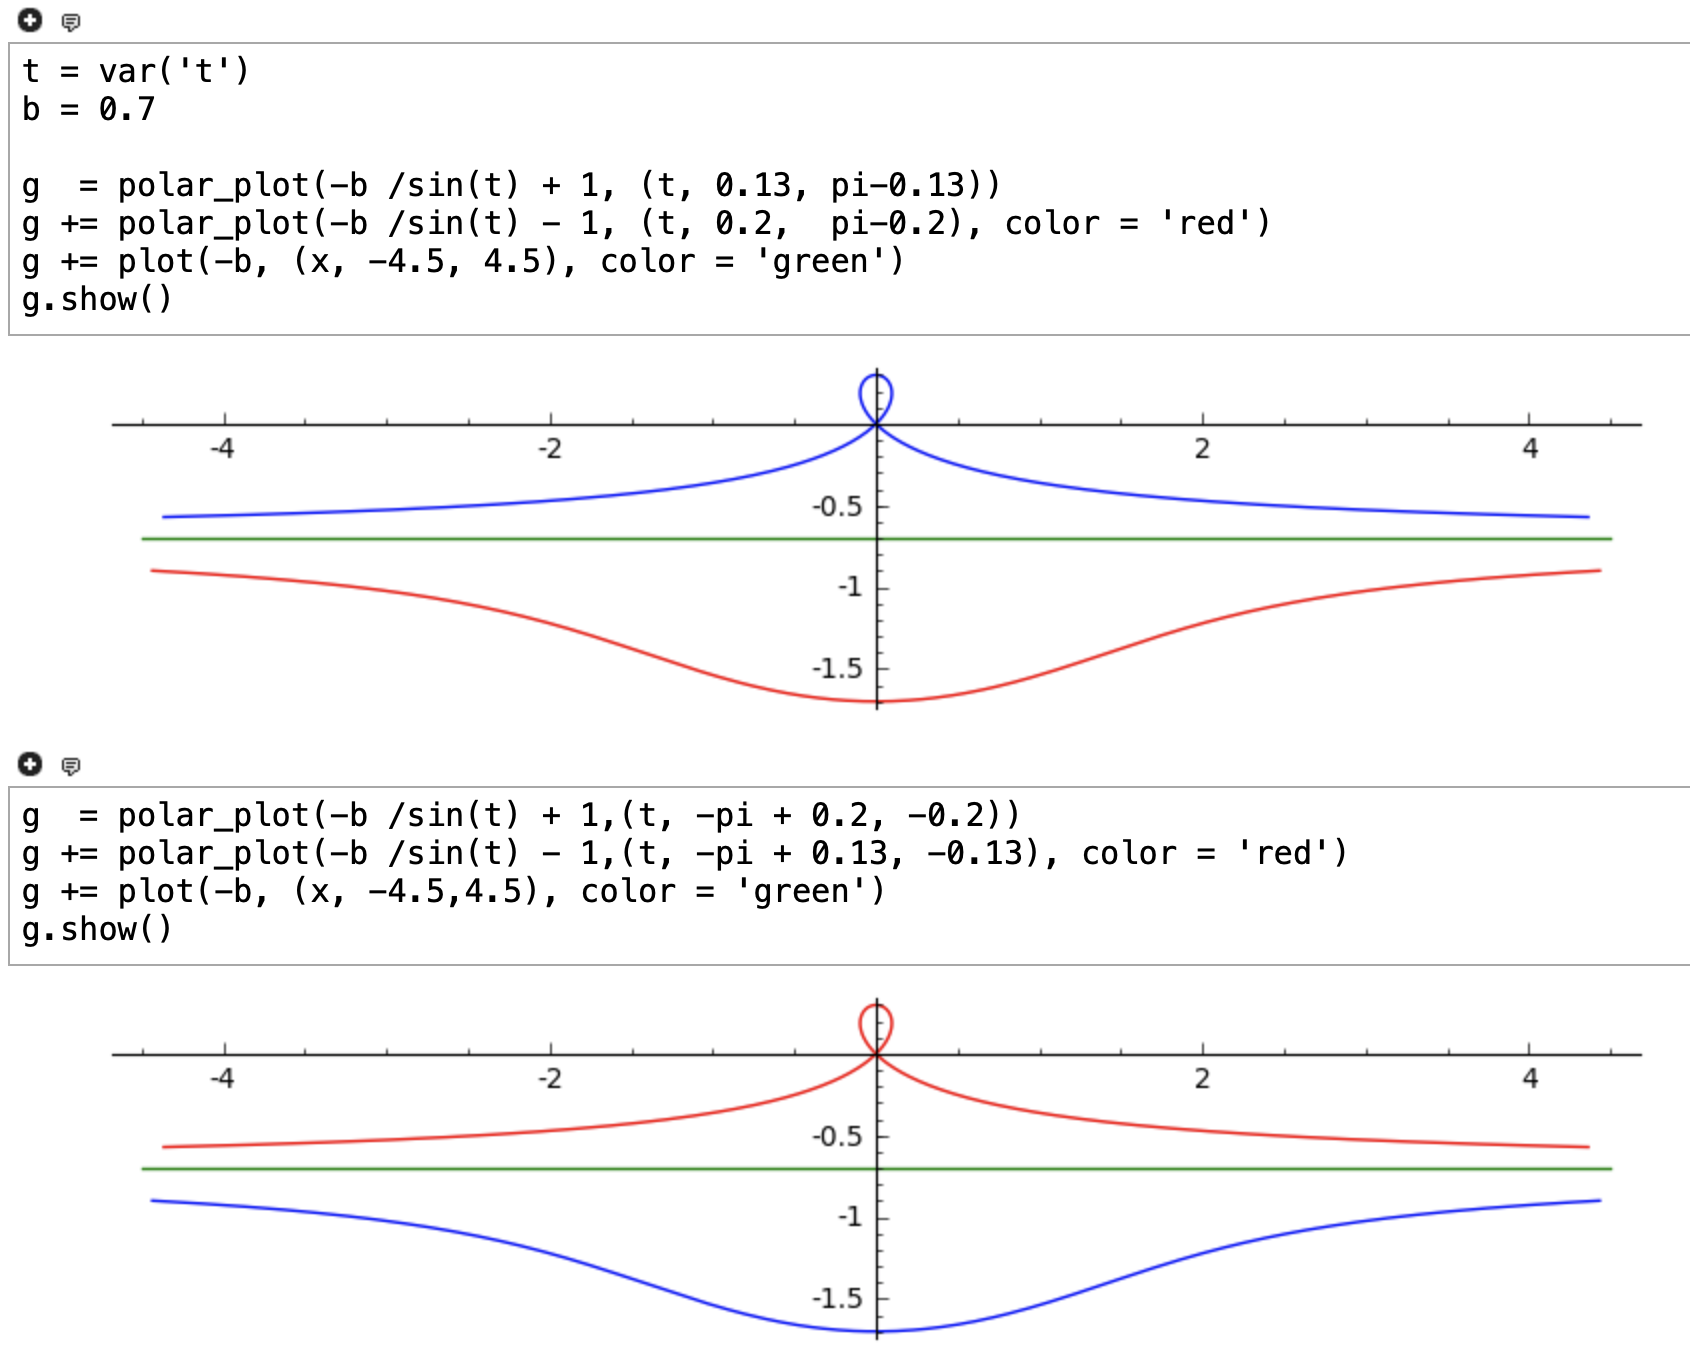
\includegraphics[width=10cm,height=8cm]{conchoid.png}
\end{center}
\end{figure}
                                                                                                                                                                                                                                                                                                                                                                                                                                                                                                                                                                                                                                                                                                                                                                                                                                                                                                                                                                                                                                                                                                                                                                                                                                                                                                                                                                                                                                                                                                                                                                                                                                                                                                                                                                                                                                                                                                                                                                                                          
So, when  $\theta$ traces $\R$, the mobile point passes through the infinity point of the curve when $\theta = k\pi, k \in \Z$, and the two parts of the curve are traced with only one of the two formulas, for instance $r = -b \csc \theta +1$.                                                                                                                                                                                                                                                                                                                                                                                                                                                                                                                                                                                                                                                                                                                                                                                                                                                                                                                                                                                                                                                                                                                                                                                                                                                                                                                                                                                                                                                                                                                                                                                                                                                                                                                                                                                                                                                                                                                                                                                                                 
\item[(d)]
Any non horizontal line $l_1$ has an equation $x = py$, where $p = 0$ or $p = 1/m$, $m$ being the slope of $l_1$.
The intersection point $R$ of $l$ with $l_1$ is $R = (-pb,-b)$, so, if $Q = (x,y)$,
\begin{align*}
Q \in  \mathscr{C}  &\iff \exists p \in \R,\ Q \in l_1 \quad \mathrm{and} \quad QR = 1\\
&\iff \exists p \in \R,\quad 
\left\{
\begin{array}{ccl}
  x&  = &  py \\
  1& = &(x + pb)^2 + (y +b)^2 
\end{array}
\right.\\
&\iff (x,y) = (0,0)\  \mathrm{or} \ \left ( x + b \frac{x}{y} \right)^2 + (y+b)^2 = 1\\
&\iff x^2(y+b)^2 + y^2(y+b)^2 = y^2\\
&\iff (x^2 + y^2)(y+b)^2 = y^2.
\end{align*}
(The polar equation gives the same Cartesian equation. For $r\ne 0$, 
\begin{align*}
\left (r + \frac{b}{\sin \theta} \right)^2 = 1 &\iff (y + b)^2 = \sin^2 \theta = \frac{y^2}{r^2}\\
&\iff (x^2 +y^2)(y+b)^2 = y^2.)
\end{align*}
The sign $-$ in the text seems to be a misprint, if the equation of $l$ is $y = -b$ (correct if the equation of $l$ is $y=b$). 
\ee
\end{proof}

\paragraph{Ex. 10.3.17}

{\it Let $P$ a point on a circle, and consider a marked ruler that goes through $P$. If we place one mark on a point $Q$ on the circle, then the other mark $R_1$ or $R_2$ traces out a curve called the lima�on of Pascal.
\be
\item[(a)] Show that the angle trisection (10.18) can be interpreted as the intersection of the line $l$ with the lima�on determined by the circle and the point $P$.
\item[(b)] Let $P =(0,0)$ and let $C$ be the circle of radius $a$ and center $(a,0)$. Show that the corresponding lima�on has polar equation
$$r = 1 + 2a \cos \theta.$$
\item[(c)] In the situation of part (b), show that the Cartesian equation of the lima�on is
$$(x^2+y^2 -2ax)^2 = x^2 + y^2.$$
\ee
}

\begin{figure}[htbp]
\begin{center}
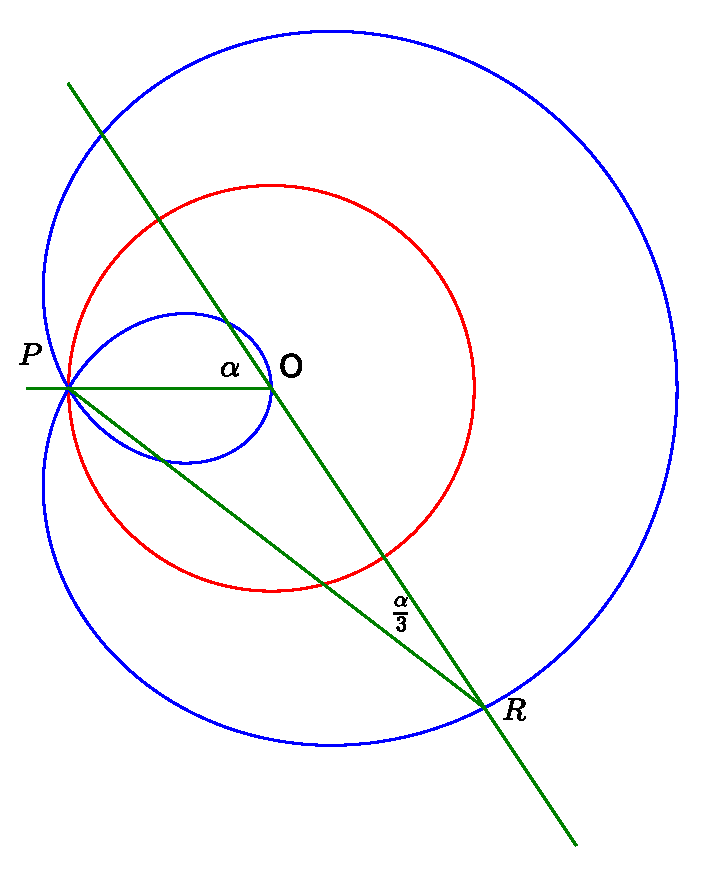
\includegraphics[width=6.5cm,height=8cm]{limacon.pdf}
\end{center}
\end{figure}
\begin{proof}
\be
\item[(a)]  As $QR = 1$, where $Q \in C$ and $R$ is on the line $(PQ)$, $R\in l$ is by definition on the lima�on determined by $P$ and $C$,

\item[(b)] Let $l_1 : y = mx$ be any nonvertical line passing through $P = (0,0)$, with $m = \tan \theta, \ -\pi / 2 <\theta < \pi/2$, so the measure of the angle between the $x$-axis and $l_1$ is $\theta$.  Let $Q =(x_Q,y_Q),Q \ne P$, be the intersection point of $l_1$ with $C$. Then $x_Q \ne 0$.

$(x_Q,y_Q)$ is solution of the system
\begin{align*}
y &= mx,\\
a^2 &=(x-a)^2 + y^2, 
\end{align*}
which gives $$y_Q = mx_Q,\qquad 0 = x_Q\, [(m^2+1)x_Q - 2a],$$ with $x_Q \ne 0$, so
$$Q = \left(\frac{2a}{m^2+1}, \frac{2am}{m^2+1}\right).$$
Since $m = \tan \theta$,
$$ Q = (2a \cos^2 \theta, 2a \sin \theta \cos \theta) = (a (\cos(2\theta)+1), a \sin(2\theta)).$$
Let $R = (r\cos \theta, r\sin \theta)$ any point of $l_1$.
Then $R$ is on the lima�on determined by $C$ and $P$ if and only if $QR = 1$ (by continuity, the points at distance 1 on the vertical tangent to the circle at point $P$ are considered to be on the lima�on):
\begin{align*}
QR = 1 &\iff 1 = (r \cos \theta - 2a \cos^2 \theta)^2 + (r \sin \theta  - 2 a \sin \theta \cos \theta)^2\\
&\iff 1 = (\cos^2 \theta + \sin^2 \theta)(r - 2 a \cos \theta)^2\\
&\iff 1 =(r - 2 a \cos \theta)^2\\
&\iff r = 1 + 2a \cos \theta \quad \mathrm{or} \quad r = -1 + 2a \cos \theta
\end{align*}
\ee
This can be interpreted geometrically. Let $P,A$ the intersection points of $C$ with the $x$-axis. As $PA$ is a diameter of $C$, the angle $\angle PQR$ is a right angle, so $PQ = 2a \cos \theta$. Therefore $PR = | PQ \pm 1| = |\pm 1 + 2a \cos \theta|$.

The lima�on is the union of the curves $C_1,C_2$ with polar equations
$$ r = 1 + 2a \cos \theta, \qquad  r = -1 + 2a \cos \theta, \qquad -\frac{\pi}{2} < \theta < \frac{\pi}{2}.$$
As $\cos(\theta + \pi) = - \cos(\theta)$, if the point $R$ with polar coordinates $(r, \theta)$ is on $C_1$, then $(-r, \theta + \pi)$ is on $C_2$. But $(r,\theta)$ and  $(-r,\theta + \pi)$ are polar coordinates of the same point!  Therefore the two curves are identical if we let $\theta$ vary in $\R$, and we obtain the complete curve if we let $\theta$ vary in $]-\pi,\pi]$ in the equation of $C_1$.

The lima�on determined by $P$ and $C$ has polar equation
$$r = 1 + 2a \cos \theta, \qquad \theta \in \R.$$

\item[(c)] Let $L$ the lima�on. By part (b), if $x \ne 0$
\begin{align*}
(x,y) \in L &\iff \exists m \in \R, 
\left\{
\begin{array}{ccl}
 y & =   & mx  \\
 1 & =  &   \left(x - \frac{2a}{m^2 + 1}\right)^2 + \left(y - \frac{2am}{m^2+1}\right) \\
\end{array}
\right.\\
 &\iff 1  =    \left(x - \frac{2a}{\frac{x^2}{y^2} + 1}\right)^2 + \left(y - \frac{2a\frac{x}{y}}{\frac{x^2}{y^2}+1}\right) \\
 &\iff x^2(x^2+y^2-2ax)^2 + y^2 (x^2+y^2-2ax)^2 = (x^2+y^2)^2\\
 &\iff (x^2 + y^2 -2ax)^2 = x^2+y^2.
\end{align*}

The two exceptional points $(0,\pm1)$ satisfy this equation, so the Cartesian equation of the lima�on is
$$L : (x^2 + y^2 -2ax)^2 = x^2+y^2.$$
(We can also obtain this equation from the polar equation $r = 1 + 2a \cos \theta$.)
\end{proof}

\paragraph{Ex. 10.3.18}

{\it A Pierpont prime is a prime $p>3$ of the form $p=2^k 3^l+1$. Prove that a regular $n$-gon can be constructed by origami (or by marked ruler or by intersections of conics) if and only if $n = 2^a 3^b p_1 \cdots p_s$ where $a,b\geq 0$ and $p_1,\ldots,p_s$ are distinct Pierpont primes. 
}

\begin{proof}
A regular $n$-gon can be constructed by origami if and only if $\zeta_n = e^{2\pi i/n}$ is an origami number (see Exercise 10.1.2, where the figures constructible by straightedge and compass are a fortiori constructible by origami). 

The splitting field of $\zeta_n$ over $\Q$ is $\Q(\zeta_n)$.
By Theorem 10.3.6, $\zeta_n$ is an origami number if and only if $[\Q(\zeta_n):\Q] = 2^a 3 ^b$ for some integers $a,b \geq 0$, and the minimal polynomial of $\zeta_n$ over $\Q$ is $\Phi_n(x)$, so $[\Q(\zeta_n):\Q]  = \deg(\Phi_n) = \phi(n)$, so
$$\zeta_n \in {\cal O} \iff \phi(n)=2^a 3^b,\ a,b \in \N.$$
\be
\item[$\bullet$] First suppose that $n=2^u3^v p_1\cdots p_s, \ u,v \geq 0$, where $p_1,\ldots,p_s$ are distinct Pierpont numbers.

Write $p_k = 2^{u_k}3^{v_k}+1, \ u_k, v_k \in \N$, for $k=1,\ldots,s$. As $2^u, 3^v, p_1,\ldots,p_s$ are relatively prime, if $u\geq 1,v \geq 1$ 
\begin{align*}
\phi(n) &= \phi(2^u) \phi(3^v) \phi(p_1)\cdots \phi(p_s) \\
	&=  (2^u- 2^{u-1}) (3^v - 3^{v-1}) (p_1-1)\cdots(p_s-1)\\
	&= 2^{u-1} ( 2 \times 3^{v-1}) (2^{u_1}3^{v_1}) \cdots (2^{u_s}3^{v_s})\\
	&= 2^a 3^b,\qquad a,b \in \N.
\end{align*}
If $u=0$, $\phi(2^u) = 1$, and if $v=0$, $\phi(3^v) = 1$. In all cases,
$$ \phi(n)=2^a 3^b,\quad a,b \in \N.$$

\item[$\bullet$] Conversely, suppose that $\phi(n)=2^a 3^b,\ a,b \geq 0$, and let the factorization of $n$ be $n = q_1^{a_1}\cdots q_s^{a_s}$, where $q_1,\ldots,q_s$ are distinct primes and the exponents $a_1,\ldots, a_s$ are all $\geq 1$. Then
$$\phi(n) = 2^a 3^b = q_1^{a_1-1}(q_1-1)\cdots q_s^{a_s-1}(q_s-1).$$
If $a_i > 1$, then $q_i \mid 2^a 3^b$, so $q_i = 2$, or $q_i=3$, and $q_i^{a_i}$ is a power of $2$ or $3$.

If $a_i=1$, then $q_i-1 \mid 2^a 3^b$, therefore $q_i - 1 = 2^{u_i} 3^{v_i}$, and so $q_i$ is a Piermont prime number, and $q_i^{a_i} = q_i =2^{u_i} 3^{v_i}+1$.

So $n = 2^a 3^b p_1 \cdots p_s$ where $a,b\geq 0$ and $p_1,\ldots,p_s$ are distinct Pierpont primes.

Conclusion: a regular $n$-gon can be constructed by origami if and only if $n = 2^a 3^b p_1 \cdots p_s$ where $a,b\geq 0$ and $p_1,\ldots,p_s$ are distinct Pierpont primes.
\ee
\end{proof}

\end{document}